
\documentclass[%
 reprint,
%superscriptaddress,
%groupedaddress,
%unsortedaddress,
%runinaddress,
%frontmatterverbose, 
%preprint,
%preprintnumbers,
nofootinbib,
%nobibnotes,
%bibnotes,
 amsmath,amssymb,
 aps,
%pra,
%prb,
%rmp,
%prstab,
%prstper,
floatfix,
]{revtex4-2}
\usepackage{gensymb}
\usepackage{textcomp}
\usepackage{lipsum}
\usepackage{graphicx}% Include figure files
\usepackage{dcolumn}% Align table columns on decimal point 


\usepackage{bm}% bold math
\usepackage{siunitx}
\DeclareSIUnit\gauss{G}
\DeclareSIUnit\erg{erg}
\DeclareMathOperator{\Rot}{rot}
\sisetup{separate-uncertainty=true}
\usepackage{tabularx}
\usepackage{amssymb}
\usepackage{amsmath}
\usepackage{relsize}
\usepackage{commath}
\usepackage{enumitem}
\usepackage{xfrac}
\usepackage{float}
\usepackage{booktabs}
\usepackage{makecell}
\usepackage{caption}
\usepackage{bm}
\usepackage{subcaption}
\DeclareSIUnit{\angstrom}{\textup{\AA}}
\usepackage{multirow}
\usepackage[version=4]{mhchem}
\usepackage[colorlinks,bookmarks=false,citecolor=blue,linkcolor=blue,urlcolor=blue]{hyperref}
%\usepackage{hyperref}% add hypertext capabilities
%\usepackage[mathlines]{lineno}% Enable numbering of text and display math
%\linenumbers\relax % Commence numbering lines

%\usepackage[showframe,%Uncomment any one of the following lines to test 
%%scale=0.7, marginratio={1:1, 2:3}, ignoreall,% default settings
%%text={7in,10in},centering,
%%margin=1.5in,
%%total={6.5in,8.75in}, top=1.2in, left=0.9in, includefoot,
%%height=10in,a5paper,hmargin={3cm,0.8in},
%]{geometry}

\begin{document}

\preprint{APS/123-QED}

\title{Compton Scattering}% Force line breaks with \\


\author{Maitrey Sharma}
\email{maitrey.sharma@niser.ac.in}
\affiliation{School of Physical Sciences, National Institute of Science Education and Research, HBNI, Jatni-752050, India}




\date{\today}% It is always \today, today,
             %  but any date may be explicitly specified

\begin{abstract}
    Compton scattering, discovered by Arthur Holly Compton, is the scattering of a photon after an interaction with a charged particle, usually an electron. This results in a decrease in energy (increase in wavelength) of the photon. In our experiment we use a MCA and Cassy Lab software to verify it. We used a mixed source to calibrate our detector, then use a Cs-137 source to study the variation of the energy of scattered photon as a function of angle for two different scattering bodies, Aluminium and Brass. Using this, we calculate the differential Compton scattering cross section (Klein-Nishina formula) and hence the calibration factor for both the bodies.
\end{abstract}

\keywords{}
\maketitle

%\tableofcontents

\section{\label{sec:level1}Introduction}
    Two of Einstein’s influential ideas introduced in 1905 were the theory of special relativity and the concept of a light quantum, which we now call a photon. Beyond 1905, Einstein went further to suggest that freely propagating electromagnetic waves consisted of photons that are particles of light in the same sense that electrons or other massive particles are particles of matter. A beam of monochromatic light of wavelength $\lambda$ (or equivalently, of frequency $f$) can be seen either as a classical wave or as a collection of photons that travel in a vacuum with one speed, c (the speed of light), and all carrying the same energy, $E_f = hf$. This idea proved useful for explaining the interactions of light with particles of matter. There were numerous such phenomena, beyond the well-known photoelectric effect and one of them was first observed by an American physicist, Arthur Holly Compton, at the Washington University in St. Louis in 1923.
    \par
    Couple of years after returning to the United States from England, Compton found that X-ray quanta scattered by free electrons had longer wavelengths and, in accordance with Planck's relation, less energy than the incoming X-rays, the surplus energy having been transferred to the electrons. This discovery demonstrated the particle concept of electromagnetic radiation. In 1923, finally Compton published his paper in \textit{Physical Review} that explained the X-ray shift by attributing particle-like momentum to photons, something Einstein had invoked for his 1905 Nobel Prize–winning explanation of the photo-electric effect. Compton himself would later be awarded the 1927 Nobel Prize in physics.
    \par
    This phenomenon, called the \textbf{\textit{Compton effect}} or \textbf{\textit{Compton scattering}} is an an example of inelastic scattering\footnote{A fundamental scattering process in which the kinetic energy of an incident particle is not conserved (in contrast to elastic scattering).} of light by a free charged particle, where the wavelength of the scattered light is different from that of the incident radiation. In Compton's original experiment (see figure (\ref{fig:original})), the energy of the X-ray photon ($\approx \SI{17}{\kilo \electronvolt}$) was very much larger than the binding energy of the atomic electron, so the electrons could be treated as being free after scattering.
    \begin{figure}
        \centering
        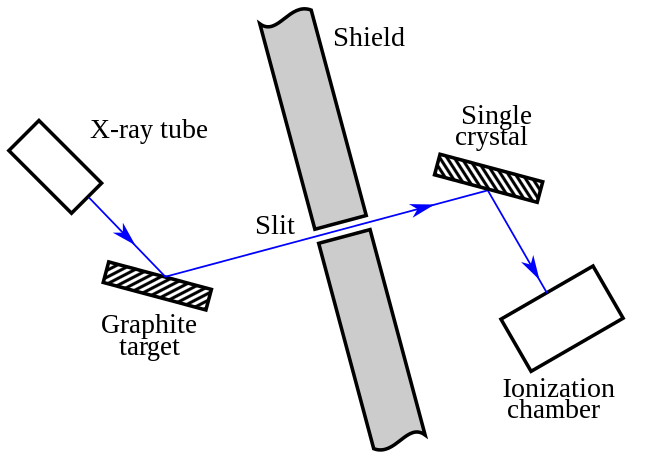
\includegraphics[scale = 0.35]{Figures/Compton-en.svg.png}
        \caption{Schematic diagram of Compton's experiment. Compton scattering occurs in the graphite target on the left. The slit passes X-ray photons scattered at a selected angle. The energy of a scattered photon is measured using Bragg scattering in the crystal on the right in conjunction with ionization chamber; the chamber could measure total energy deposited over time, not the energy of single scattered photons.}
        \label{fig:original}
    \end{figure}
    \par
    The effect is significant because it demonstrates that light cannot be explained purely as a wave phenomenon. Thomson scattering, the classical theory of an electromagnetic wave scattered by charged particles, cannot explain shifts in wavelength at low intensity: classically, light of sufficient intensity for the electric field to accelerate a charged particle to a relativistic speed will cause radiation-pressure recoil and an associated Doppler shift of the scattered light, but the effect would become arbitrarily small at sufficiently low light intensities \textit{regardless of wavelength}. Thus, if we are to explain low-intensity Compton scattering, light must behave as if it consists of particles. Or the assumption that the electron can be treated as free is invalid resulting in the effectively infinite electron mass equal to the nuclear mass. Compton's experiment convinced physicists that light can be treated as a stream of particle-like objects (quanta called photons), whose energy is proportional to the light wave's frequency.
    
\section{Aim}
    Our primary objectives in this experiment are
    \begin{enumerate}
        \item Energy calibration of scintillation detector,
        \item Determination of change in wavelength of the scattered gamma radiation as a function of the scattering angle,
        \item Determination of the differential cross-section using Klein-Nishina formula and calculation of calibration factor.
    \end{enumerate}
    
\section{Apparatus}
    The apparatus used in this experiment are
    \begin{enumerate}
        \item Cs-137 radioactive gamma source,
        \item Mixed preparation radioactive source for calibration (Am-241 and Cs-137),
        \begin{figure}
            \centering
            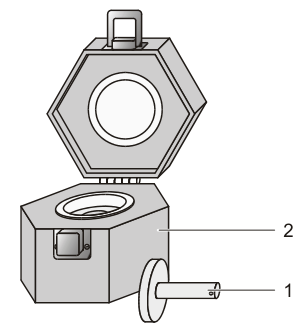
\includegraphics{Figures/box.png}
            \caption{Cs-137 preparation: Safety container (1) and Radioactive preparation (2)}
            \label{fig:box}
        \end{figure}
        \item Source holder in form of a lead block with a hole of $\SI{12}{\milli \metre}$ diameter at the centre to accommodate radioactive sources. Additional blind hole for inserting a steel pin as angular direction indicator,
        \item NaI scintillation detector and its holder with lead shielding for defined direction of incoming gamma radiation,
        \item High voltage power supply ($\SI{1.5}{\kilo \volt}$),
        \item Cylindrical pure aluminium/copper rod as centre of scattering,
        \item Additional lead shielding (movable) to reduce the intensity of unscattered gamma radiation, particularly for small scattering angles and short distances between source, scatterer and detector,
        \item Multichannel analyzer (256 channels) and related software in a desktop PC,
        \item Experimental panel with graduated angular scale.
    \end{enumerate}

\section{Experiment description}
    The complete experimental set up is shown in (figure (\ref{fig:setup})) and can be visualized in the following sequence. A radioactive Cs-137 source produces $\SI{662}{\kilo \electronvolt}$ $\gamma$-rays which can escape the shielded cavity only through a small hole. The beam is collimated and reaches an aluminium rod (the target or scatterer). Some portion of the $\gamma$-rays are scattered by the electrons in the target which are detected and counted by the scintillator detector. The detected signal is further processed by an MCA and the complete spectrum is displayed on the computer. By placing the source at different angles on the experimental angular panel, the scattered radiations are collected to study the angular dependence of Compton scattering.
    \begin{figure}
        \centering
        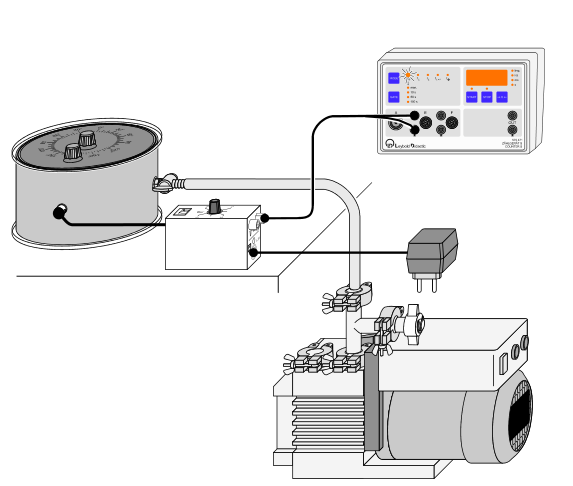
\includegraphics[scale = 0.39]{Figures/setup.png}
        \caption{Experimental set up for Compton scattering experiment consisting of 1. Source holder, 2. Scintillator detector with lead shielding, 3. High voltage supply, 4. Scatterer, 5. Additional movable shielding, 6. MCA and 7. a Experimental panel with angular scale}
        \label{fig:setup}
    \end{figure}
    \begin{figure}
        \centering
        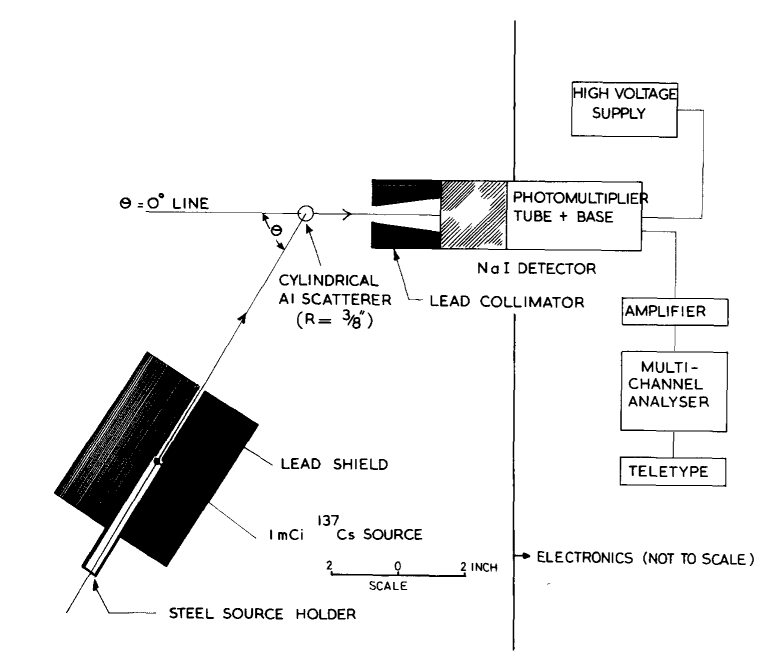
\includegraphics[scale = 0.45]{Figures/schematic.png}
        \caption{Experimental arrangement for the study of Compton scattering.}
        \label{fig:schematic}
    \end{figure}

\section{Theory}
    In his 1923 paper, Compton came up with the mathematical relation in order to explain the wavelength shift.
    \begin{equation}
    \label{eq:shift}
        \lambda_f - \lambda_i = \Delta \lambda = \dfrac{h}{m_e c}(1 \cos \theta)
    \end{equation}
    \begin{figure}
        \centering
        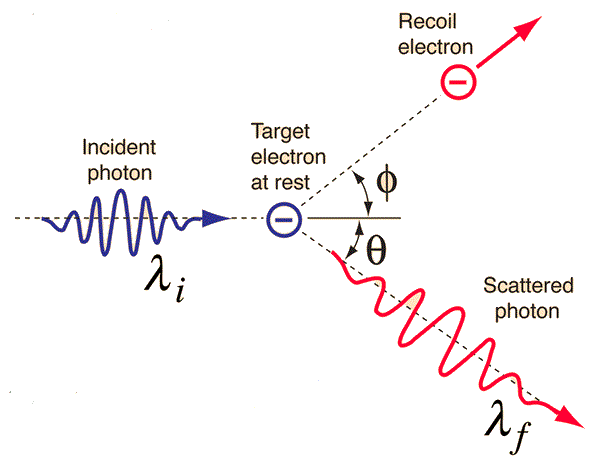
\includegraphics[scale = 0.37]{Figures/Compton_feynman.png}
        \caption{A photon of wavelength $\lambda_i$ comes in from the left, collides with a target at rest, and a new photon of wavelength $\lambda_f$ emerges at an angle $\theta$ . The target recoils, carrying away an angle-dependent amount of the incident energy.}
        \label{fig:compton}
    \end{figure}
    where $\lambda_i$ and $\lambda_f$ are wavelengths of incident and scattered photon respectively, $h$ is the Planck’s constant, $m_e$ is the rest mass of electron, $c$ is the velocity of light, $\theta$ and $\phi$ are angles of scattered photon and recoil electron respectively (figure (\ref{fig:compton})). The value of ($h/m_e c = \SI{0.02426}{\angstrom}$) is called Compton wavelength of electron. In terms of energy equation (\ref{eq:shift}) can be rewritten as
    \begin{equation}
        E_f = E_i \dfrac{1}{1 + \big( \gamma (1 - \cos \theta) \big)}
    \end{equation}
    where $E_i$ and $E_f$ are energy of incident and scattered photon respectively and $\gamma = E_i/m_e c^2$. From here we can write
    \begin{equation}
        E_i = E_f \dfrac{1}{1 - \Bigg( \dfrac{E_{f} (1 - \cos \theta)}{m_e c^2}  \Bigg)}
    \end{equation}
    \par 
    For high energy photons with ($\lambda \ll \SI{0.02}{\angstrom}$ or $E \gg \SI{511}{\kilo \electronvolt}$) wavelength of the scattered radiation is always of the order of the Compton wavelength whereas for low energy photons ($E \gg \SI{511}{\kilo \electronvolt}$) the Compton shift is very small. In other words, in non-relativistic energy regime, Compton scattering results approaches the results predicted by classical Thompson scattering.
    \par
    The Klein–Nishina formula gives the differential cross section (i.e. the \textit{likelihood} and angular distribution) of photons scattered from a single free electron, calculated in the lowest order of quantum electrodynamics. It was first derived in 1928 by Oskar Klein and Yoshio Nishina, constituting one of the first successful applications of the Dirac equation. This formula can be used to describe the Compton scattering as

    \begin{equation}
    \label{eq:nishi}
        \begin{split}
            \dfrac{d \sigma}{d \Omega} &= r_0^2 \Bigg( \dfrac{1 + \cos^2 \theta}{2} \Bigg) \Bigg( \dfrac{1}{\big( 1 + \gamma (1 - \cos \theta)^2 \big)} \Bigg) \\ 
            & \times \Bigg[ \dfrac{\gamma^2 (1 - \cos \theta)^2}{\big( 1 + \cos^2 \theta  \big) \big( 1 + \gamma (1 - \cos \theta) \big)} + 1 \Bigg]
        \end{split}
    \end{equation}

    Here, $r_0 = (e_0/4 \pi \epsilon_0 m c^2$) is the is the classical electron radius and has the value $r_0 = \SI{2.818e-15}{\metre}$. This result is for the cross section averaged over all incoming photon polarizations. By integrating equation (\ref{eq:nishi}) over all angles, the total cross section can be obtained.
    \par
    In our experiment gamma rays from a Cesium-137 source are used as the source of photons that are scattered. Difference in the incident and scattered energy and wavelength of the photons is determined by a calibrated scintillation detector placed at different scattering angles. The relative intensities $I_{\theta}$ of the scatter radiation peaks can be compared with the predictions of the Klein-Nishina formula for the differential effective cross section ($\frac{d \sigma}{d \Omega}$) by calculating the calibration factor $C$ using the formula below
    \begin{equation}
    \label{eq:calib}
        C = \dfrac{1}{n} \sum_{\theta = 0}^{n} \dfrac{I_{\theta}}{\frac{d \sigma}{d \Omega}}
    \end{equation}
    \par
    The area under the curve of the peak in the energy spectrum acquisition plot will yield the value of $I_{theta}$.

\section{Observations and Evaluation}
    \subsection{Aluminium as the scattering body}
    The calibration curve is given in figure (\ref{fig:al-2}). The energy spectrum acquisition at various angles is given in figure (\ref{fig:al-1}). The corresponding plot of scattered energy $E_f$ against scattering angle $\theta$ is given in figure (\ref{fig:al-3}). The scattered energy, the differential cross-section, intensities and calibration factor are tabulated in table (\ref{tab:al}). The plot of differential cross-section with scattering angle is given in figure (\ref{fig:al-C}).
    \par
    From the table (\ref{tab:al}), the average calibration factor using equation (\ref{eq:calib}) is
    \begin{equation}
        \begin{split}
            C_{Al} &= \dfrac{1}{n} \sum_{\theta = 0}^{n} \dfrac{I_{\theta}}{\frac{d \sigma}{d \Omega}} \\
            &= \dfrac{1}{6} \times 2.741 \times 10^{33} \\
            &= \boxed{4.569 \times 10^{32}}
        \end{split}
    \end{equation}

    
    \begin{figure}
        \centering
        \begin{subfigure}[b]{0.48\textwidth}
            \centering
            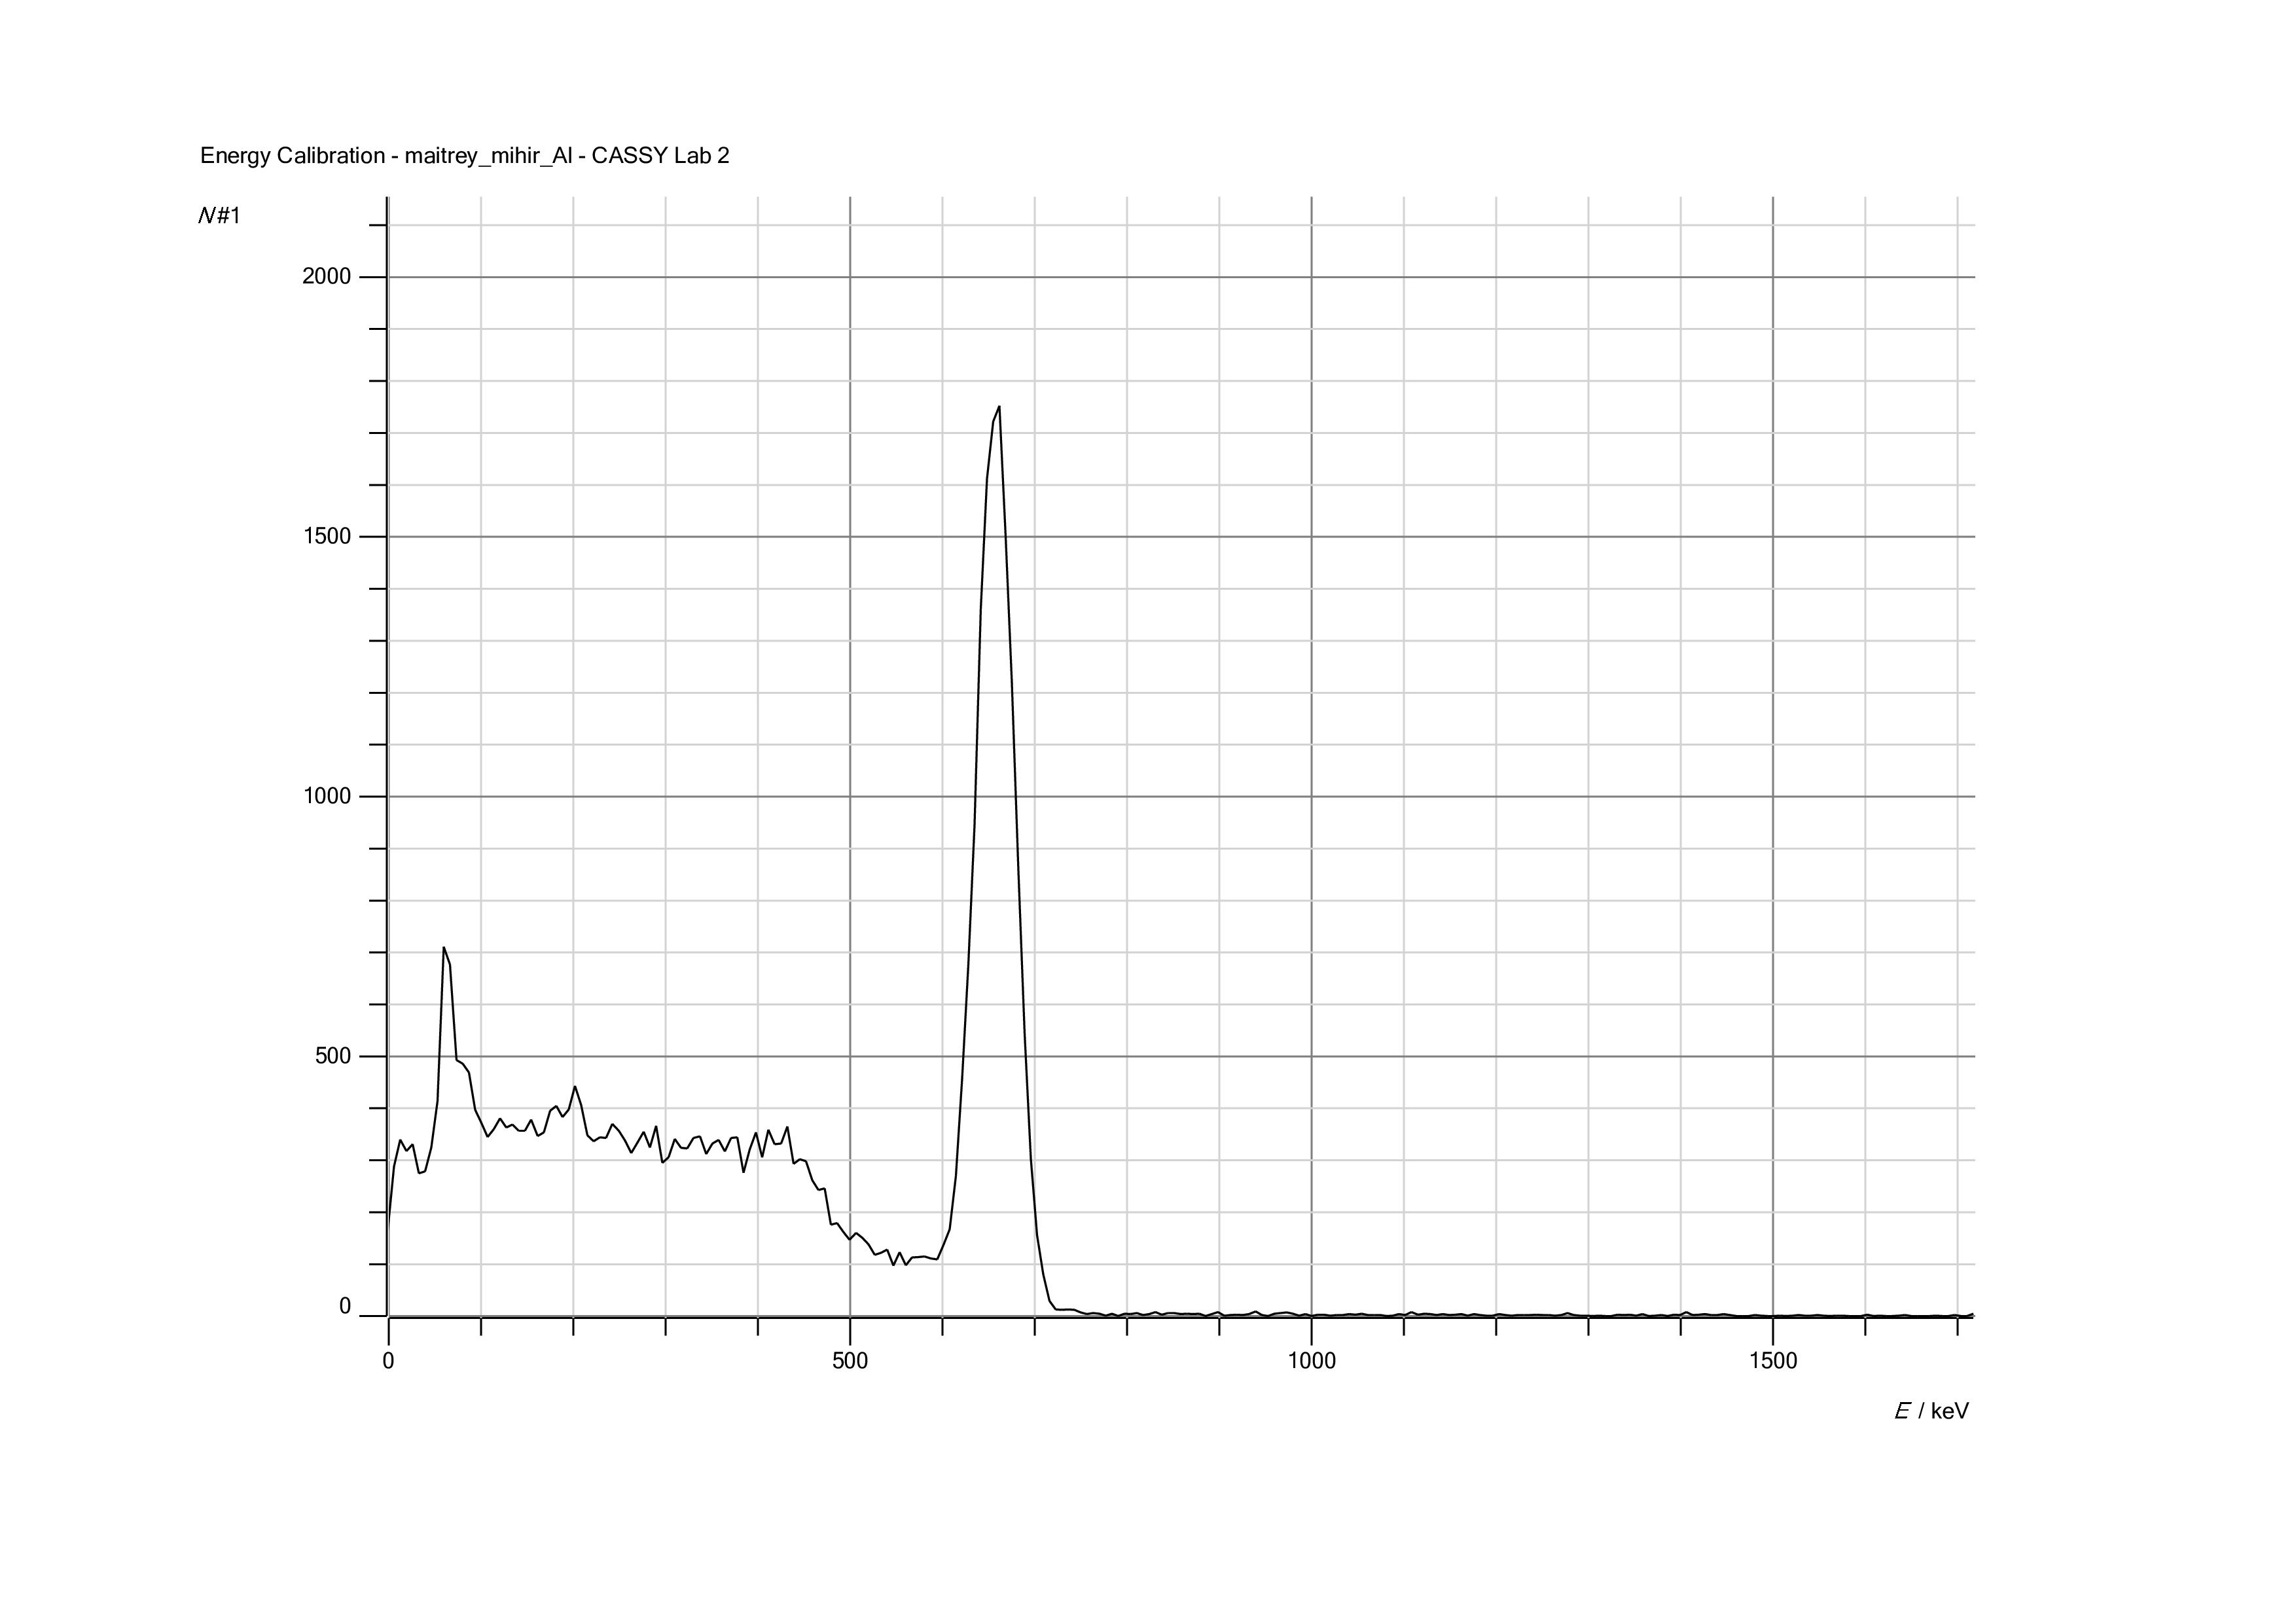
\includegraphics[scale = 0.069]{Figures/calib_Al_diagram (pdf.io).png}
            \caption{Calibration plot}
            \label{fig:al-2}
        \end{subfigure}
        \begin{subfigure}[b]{0.48\textwidth}
            \centering
            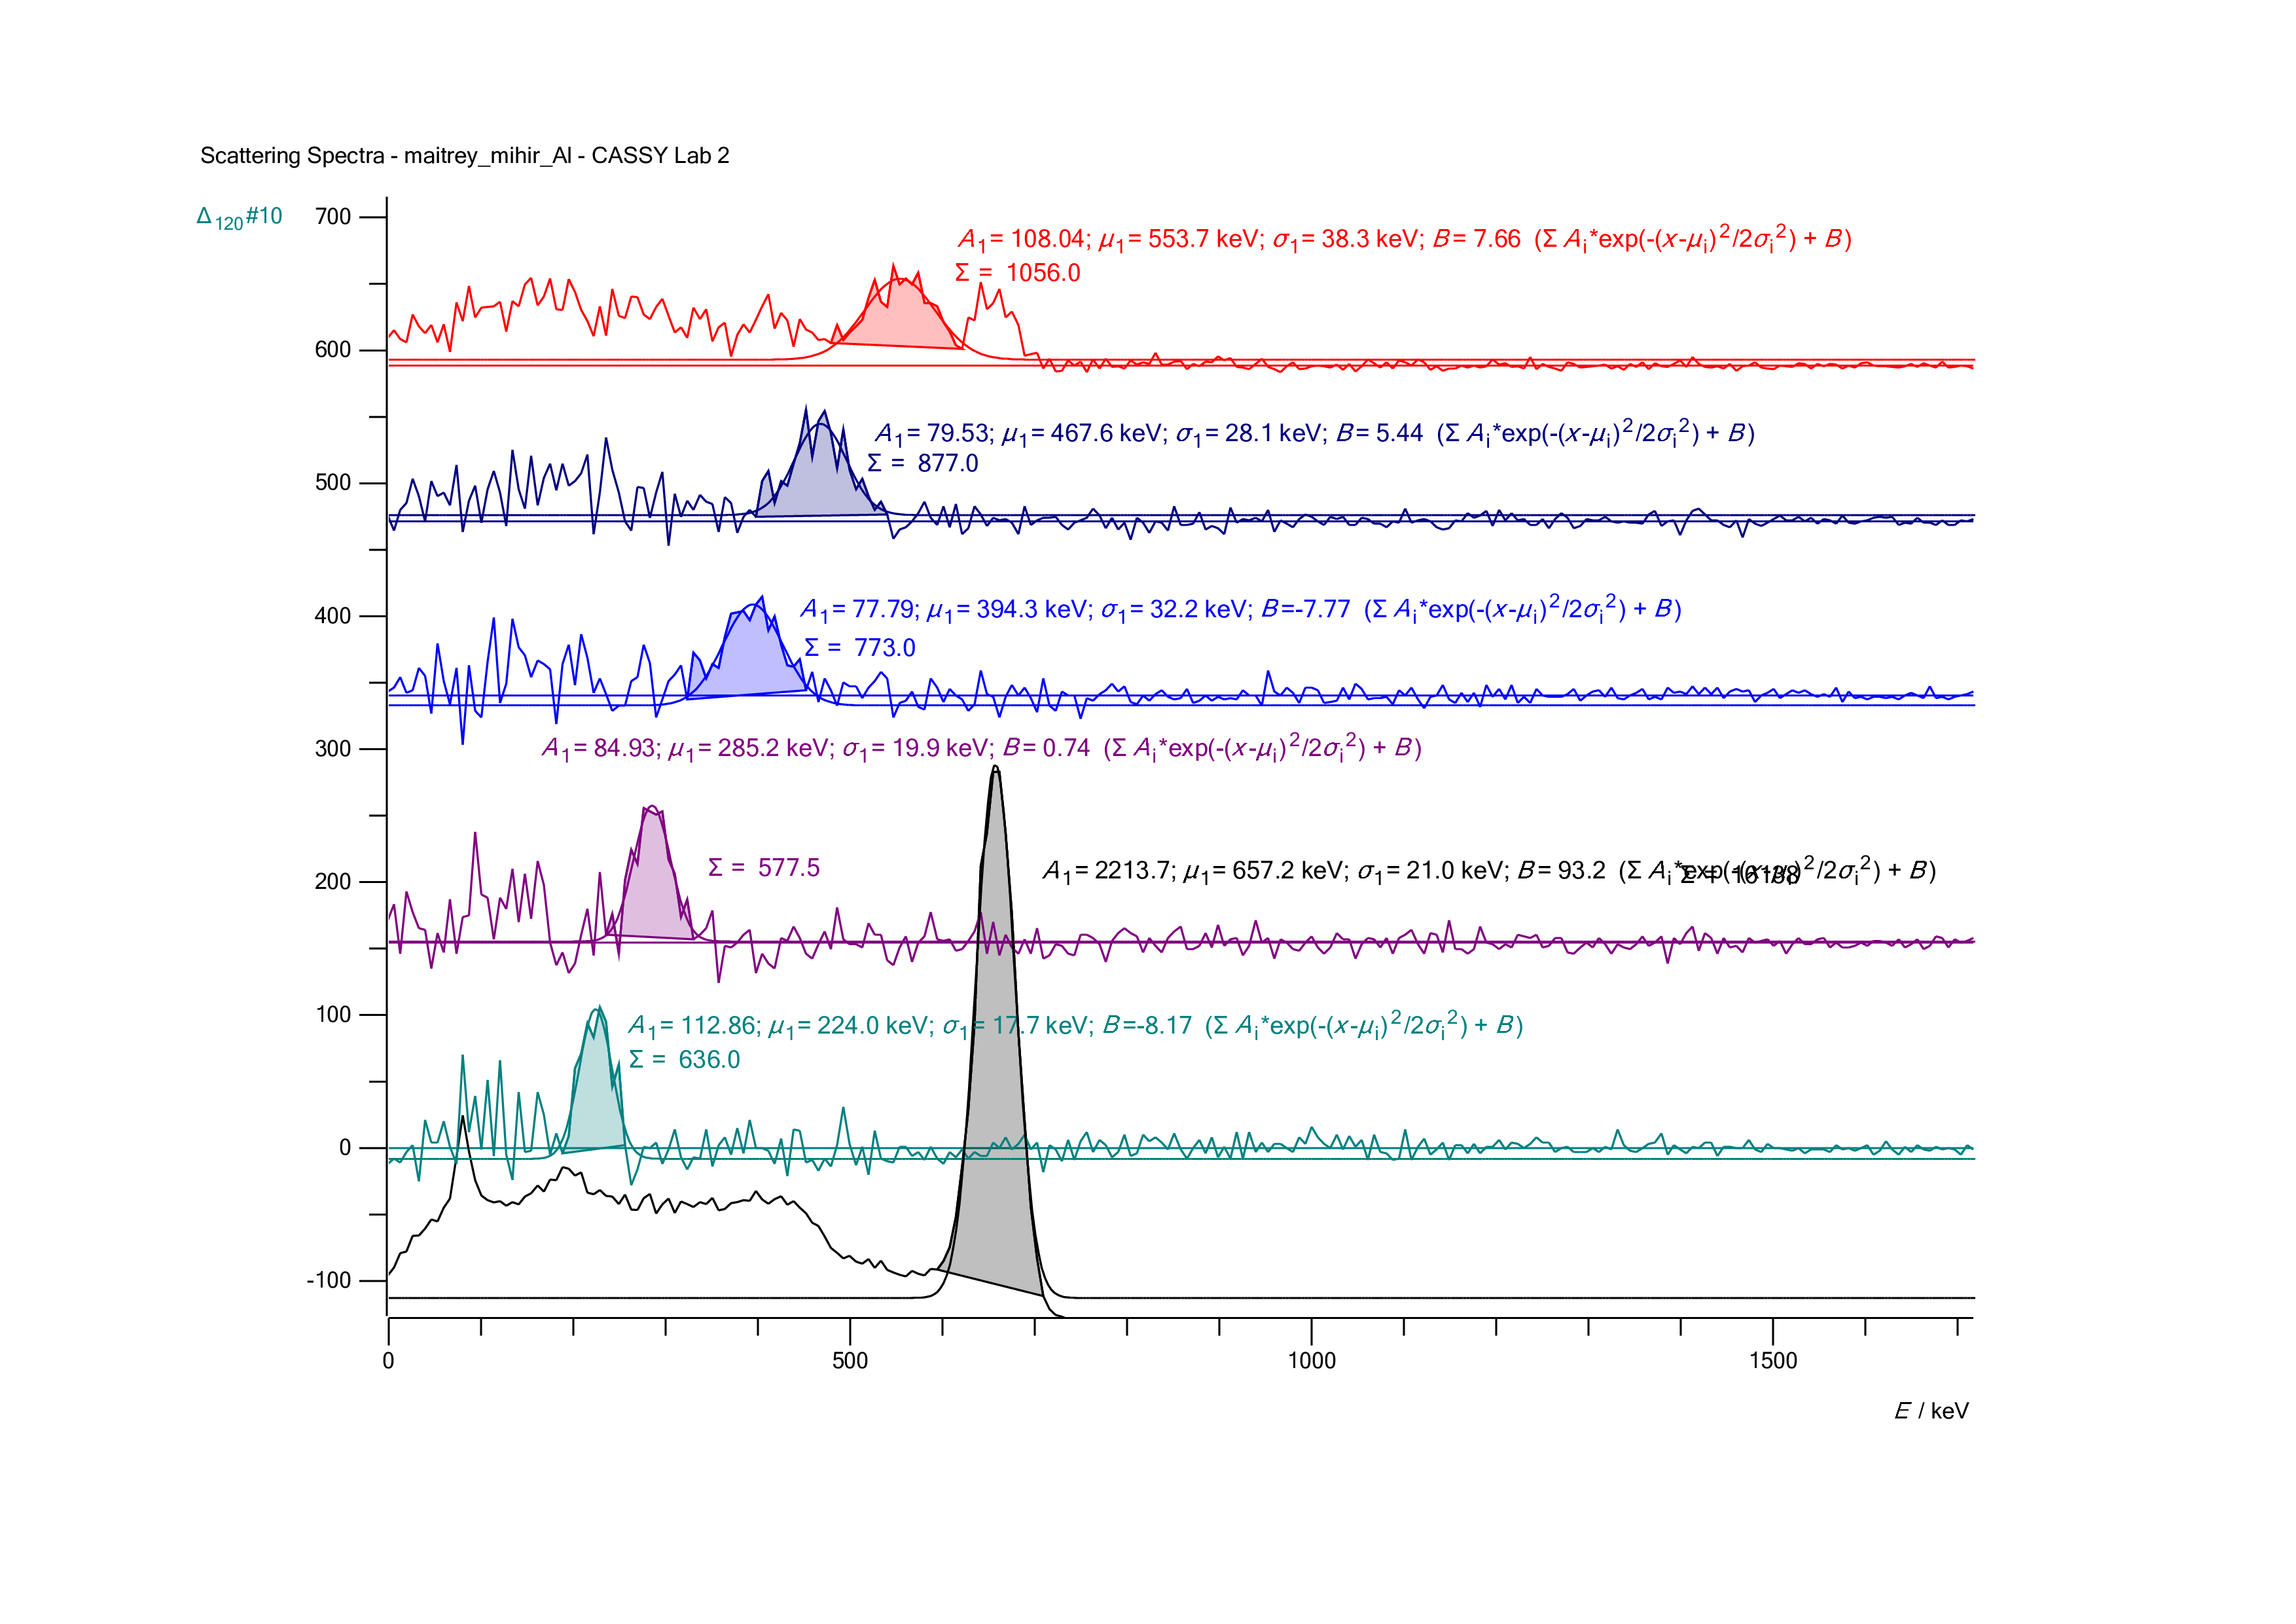
\includegraphics[scale = 0.069]{Figures/diagram_Al (pdf.io).png}
            \caption{Energy spectrum acquisition plot}
            \label{fig:al-1}
        \end{subfigure}
        \hfill
        \hfill
        \begin{subfigure}[b]{0.48\textwidth}
            \centering
            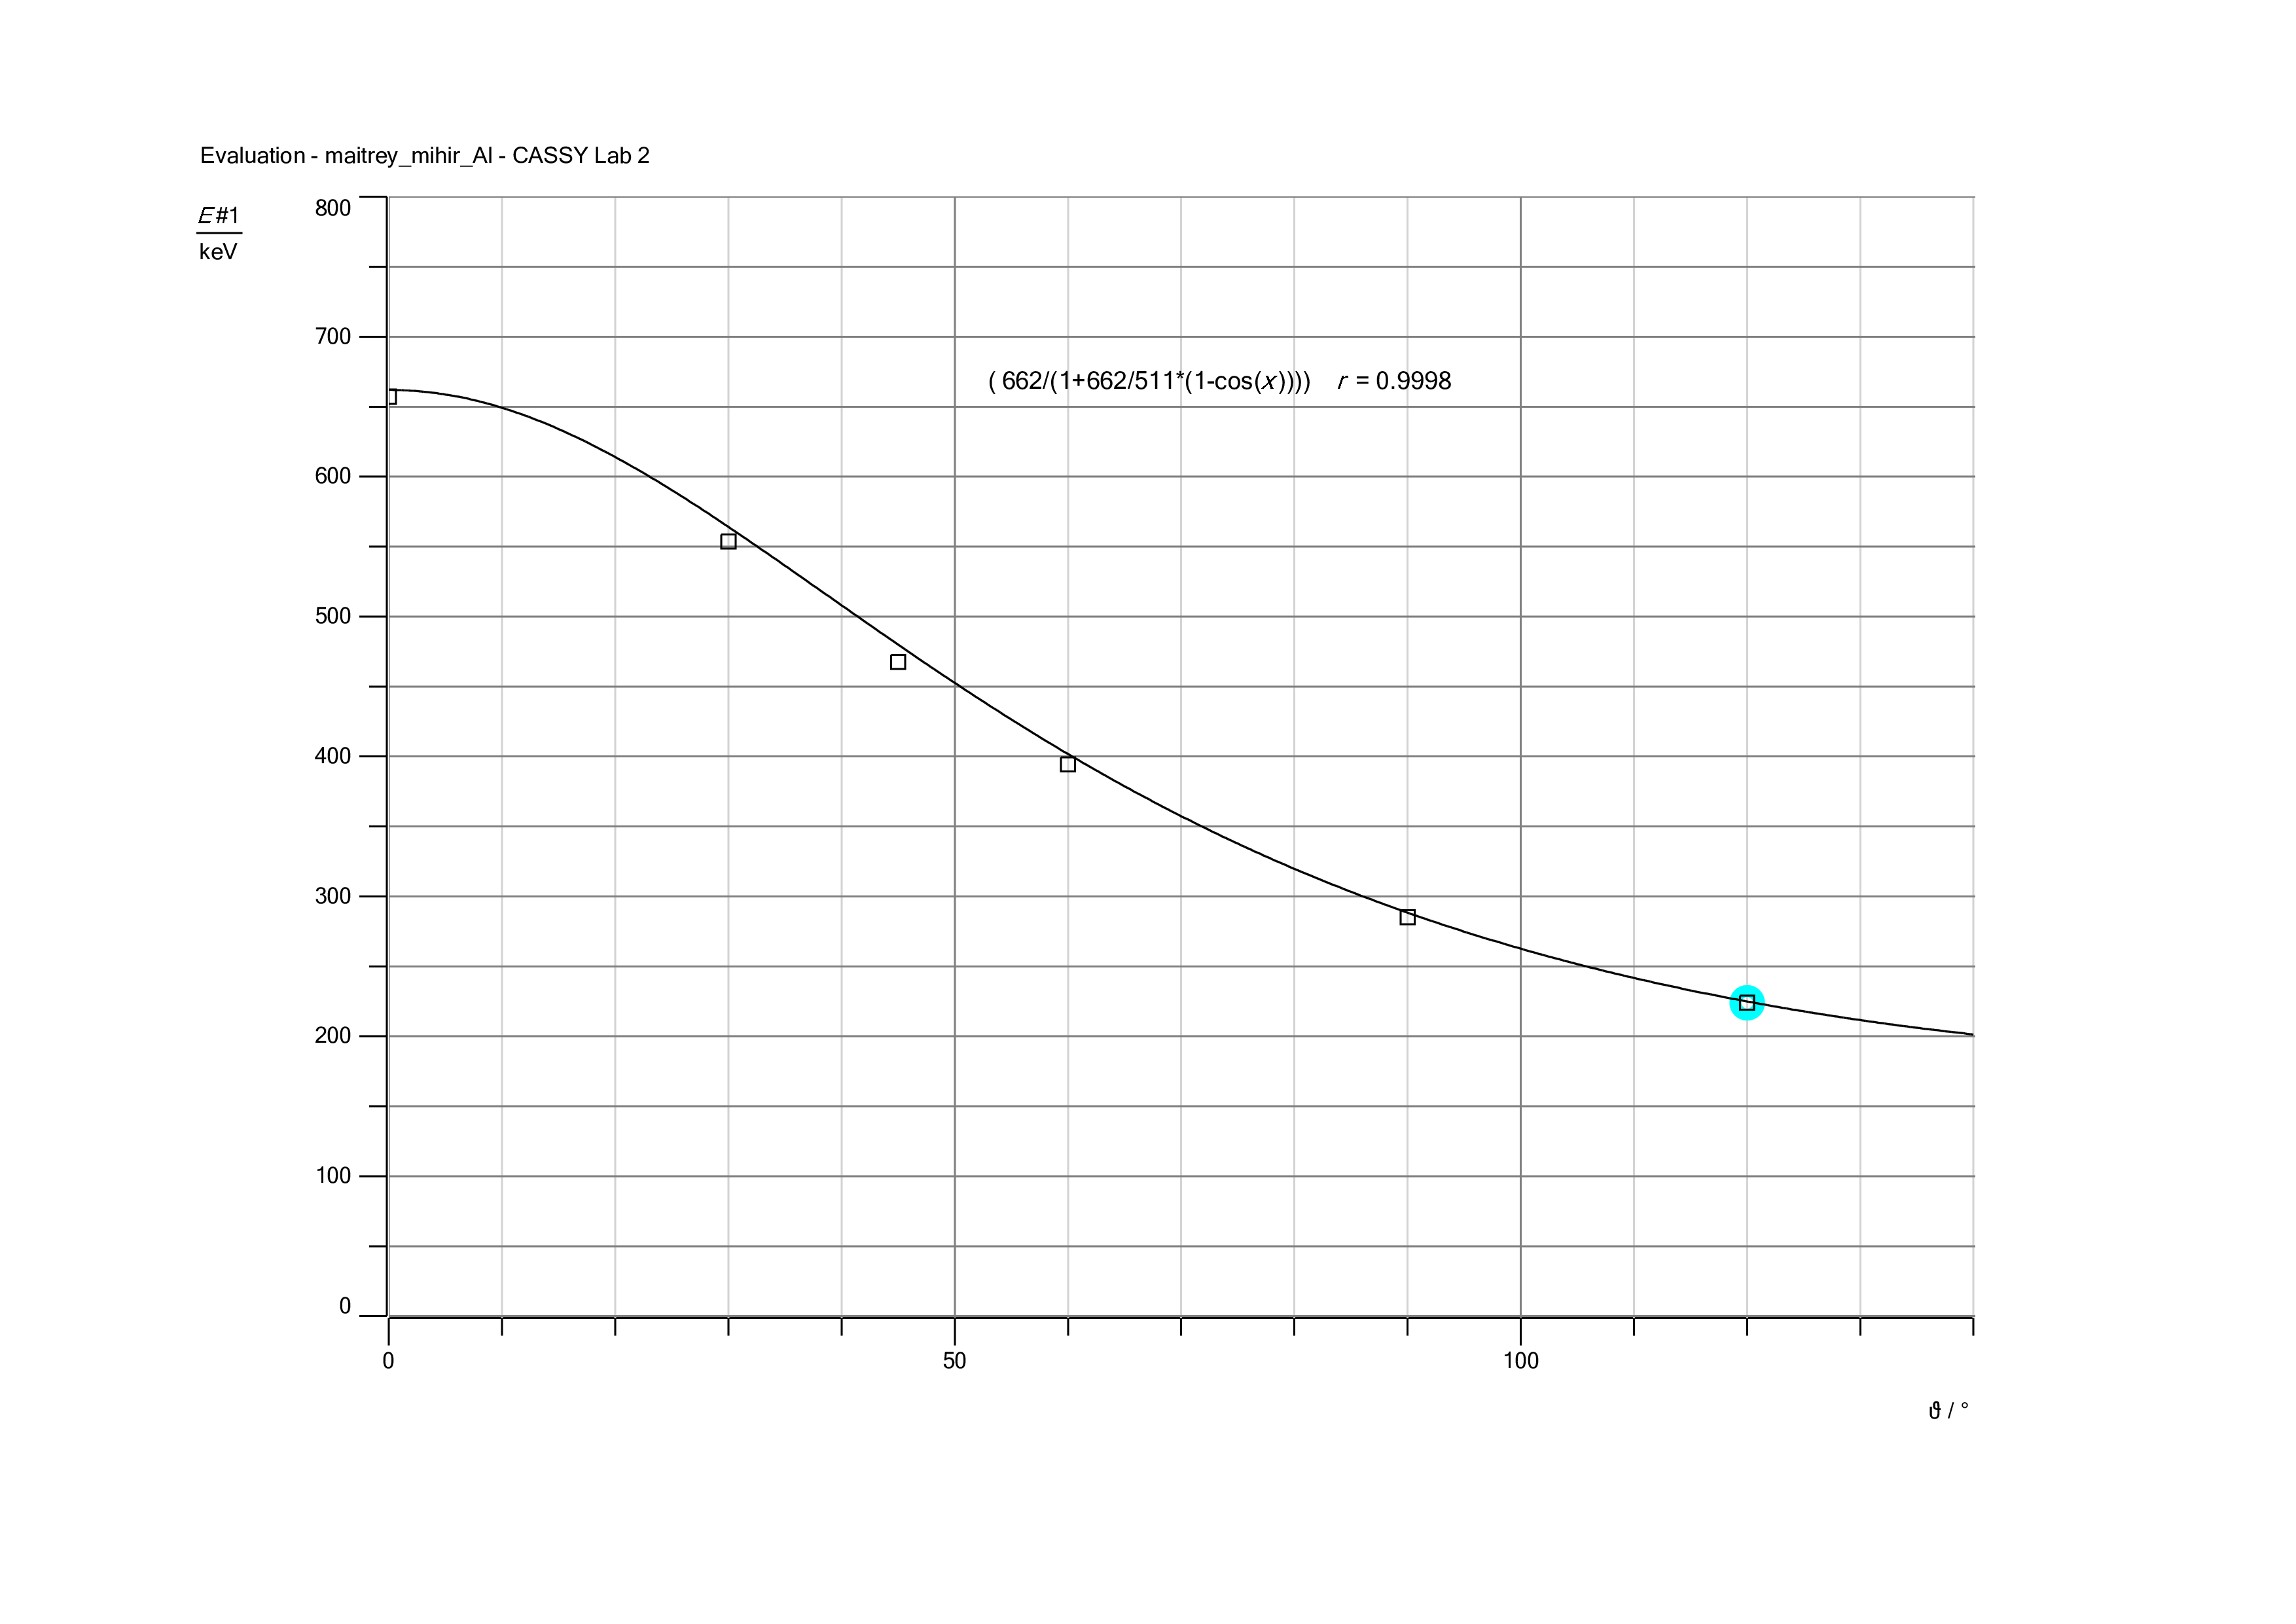
\includegraphics[scale = 0.069]{Figures/eval_Al_diagram.png}
            \caption{Plot of scattered energy with scattering angle}
            \label{fig:al-3}
        \end{subfigure}
            \caption{Calibration, energy spectrum acquisition and scattered energy versus scattering angle plots for Aluminium}
            \label{fig:al}
    \end{figure}
    \begin{table*}[]
    \caption{The scattered energy, the differential cross-section, intensities and the calibration factor for Aluminium. The intensities are the area under the curve of the peak in the energy spectrum acquisition plots given in figure (\ref{fig:al-1})}
    \label{tab:al}
    \setlength{\tabcolsep}{15pt}
    \begin{tabular}{@{}ccccccc@{}}
    \toprule
    \begin{tabular}[c]{@{}c@{}}$\bm{\theta}$\\ (degrees)\end{tabular} &
    \begin{tabular}[c]{@{}c@{}}$\bm{E_f}$\\ ($\si{\kilo \electronvolt}$)\end{tabular} & 
    \begin{tabular}[c]{@{}c@{}}$\bm{E_f}$\\ ($\si{\joule}$)\end{tabular} &
    \begin{tabular}[c]{@{}c@{}}$\bm{\gamma}$\\ ($\si{\joule \second \squared \per \kilogram \per \metre}$) \end{tabular} & 
    \begin{tabular}[c]{@{}c@{}}\textbf{Differential}\\ \textbf{cross-section}\end{tabular} & $\bm{I_{\theta}}$ & 
    \begin{tabular}[c]{@{}c@{}}$\bm{C_{\theta}}$\\ ($\si{\steradian \per \metre \squared}$)\end{tabular} \\ \midrule
    0 & 657.2 & $1.052 \times 10^{-19}$ & $1.284 \times 10^{-06}$ & $7.998 \times 10^{-30}$ & 16138 & $2.018 \times 10^{33}$ \\
    30 & 553.7 &  $8.859 \times 10^{-20}$ & $1.082 \times 10^{-06}$ & $6.998 \times 10^{-30}$ & 1056 & $1.509 \times 10^{32}$ \\
    45 & 467.6 &  $7.482 \times 10^{-20}$ & $9.135 \times 10^{-07}$ & $5.998 \times 10^{-30}$ & 877 & $1.462 \times 10^{32}$ \\
    60 & 394.3 &  $6.309 \times 10^{-20}$ & $7.703 \times 10^{-07}$ & $4.998 \times 10^{-30}$ & 773 & $1.546 \times 10^{32}$ \\
    90 & 285.2 &  $4.563 \times 10^{-20}$ & $5.572 \times 10^{-07}$ & $3.999 \times 10^{-30}$ & 577.5 & $1.444 \times 10^{32}$ \\
    120 & 224 &  $3.584 \times 10^{-20}$ & $4.376 \times 10^{-07}$ & $4.998 \times 10^{-30}$ & 636 & $1.272 \times 10^{32}$ \\ \bottomrule
    \end{tabular}
    \end{table*}
    \begin{figure}
        \centering
        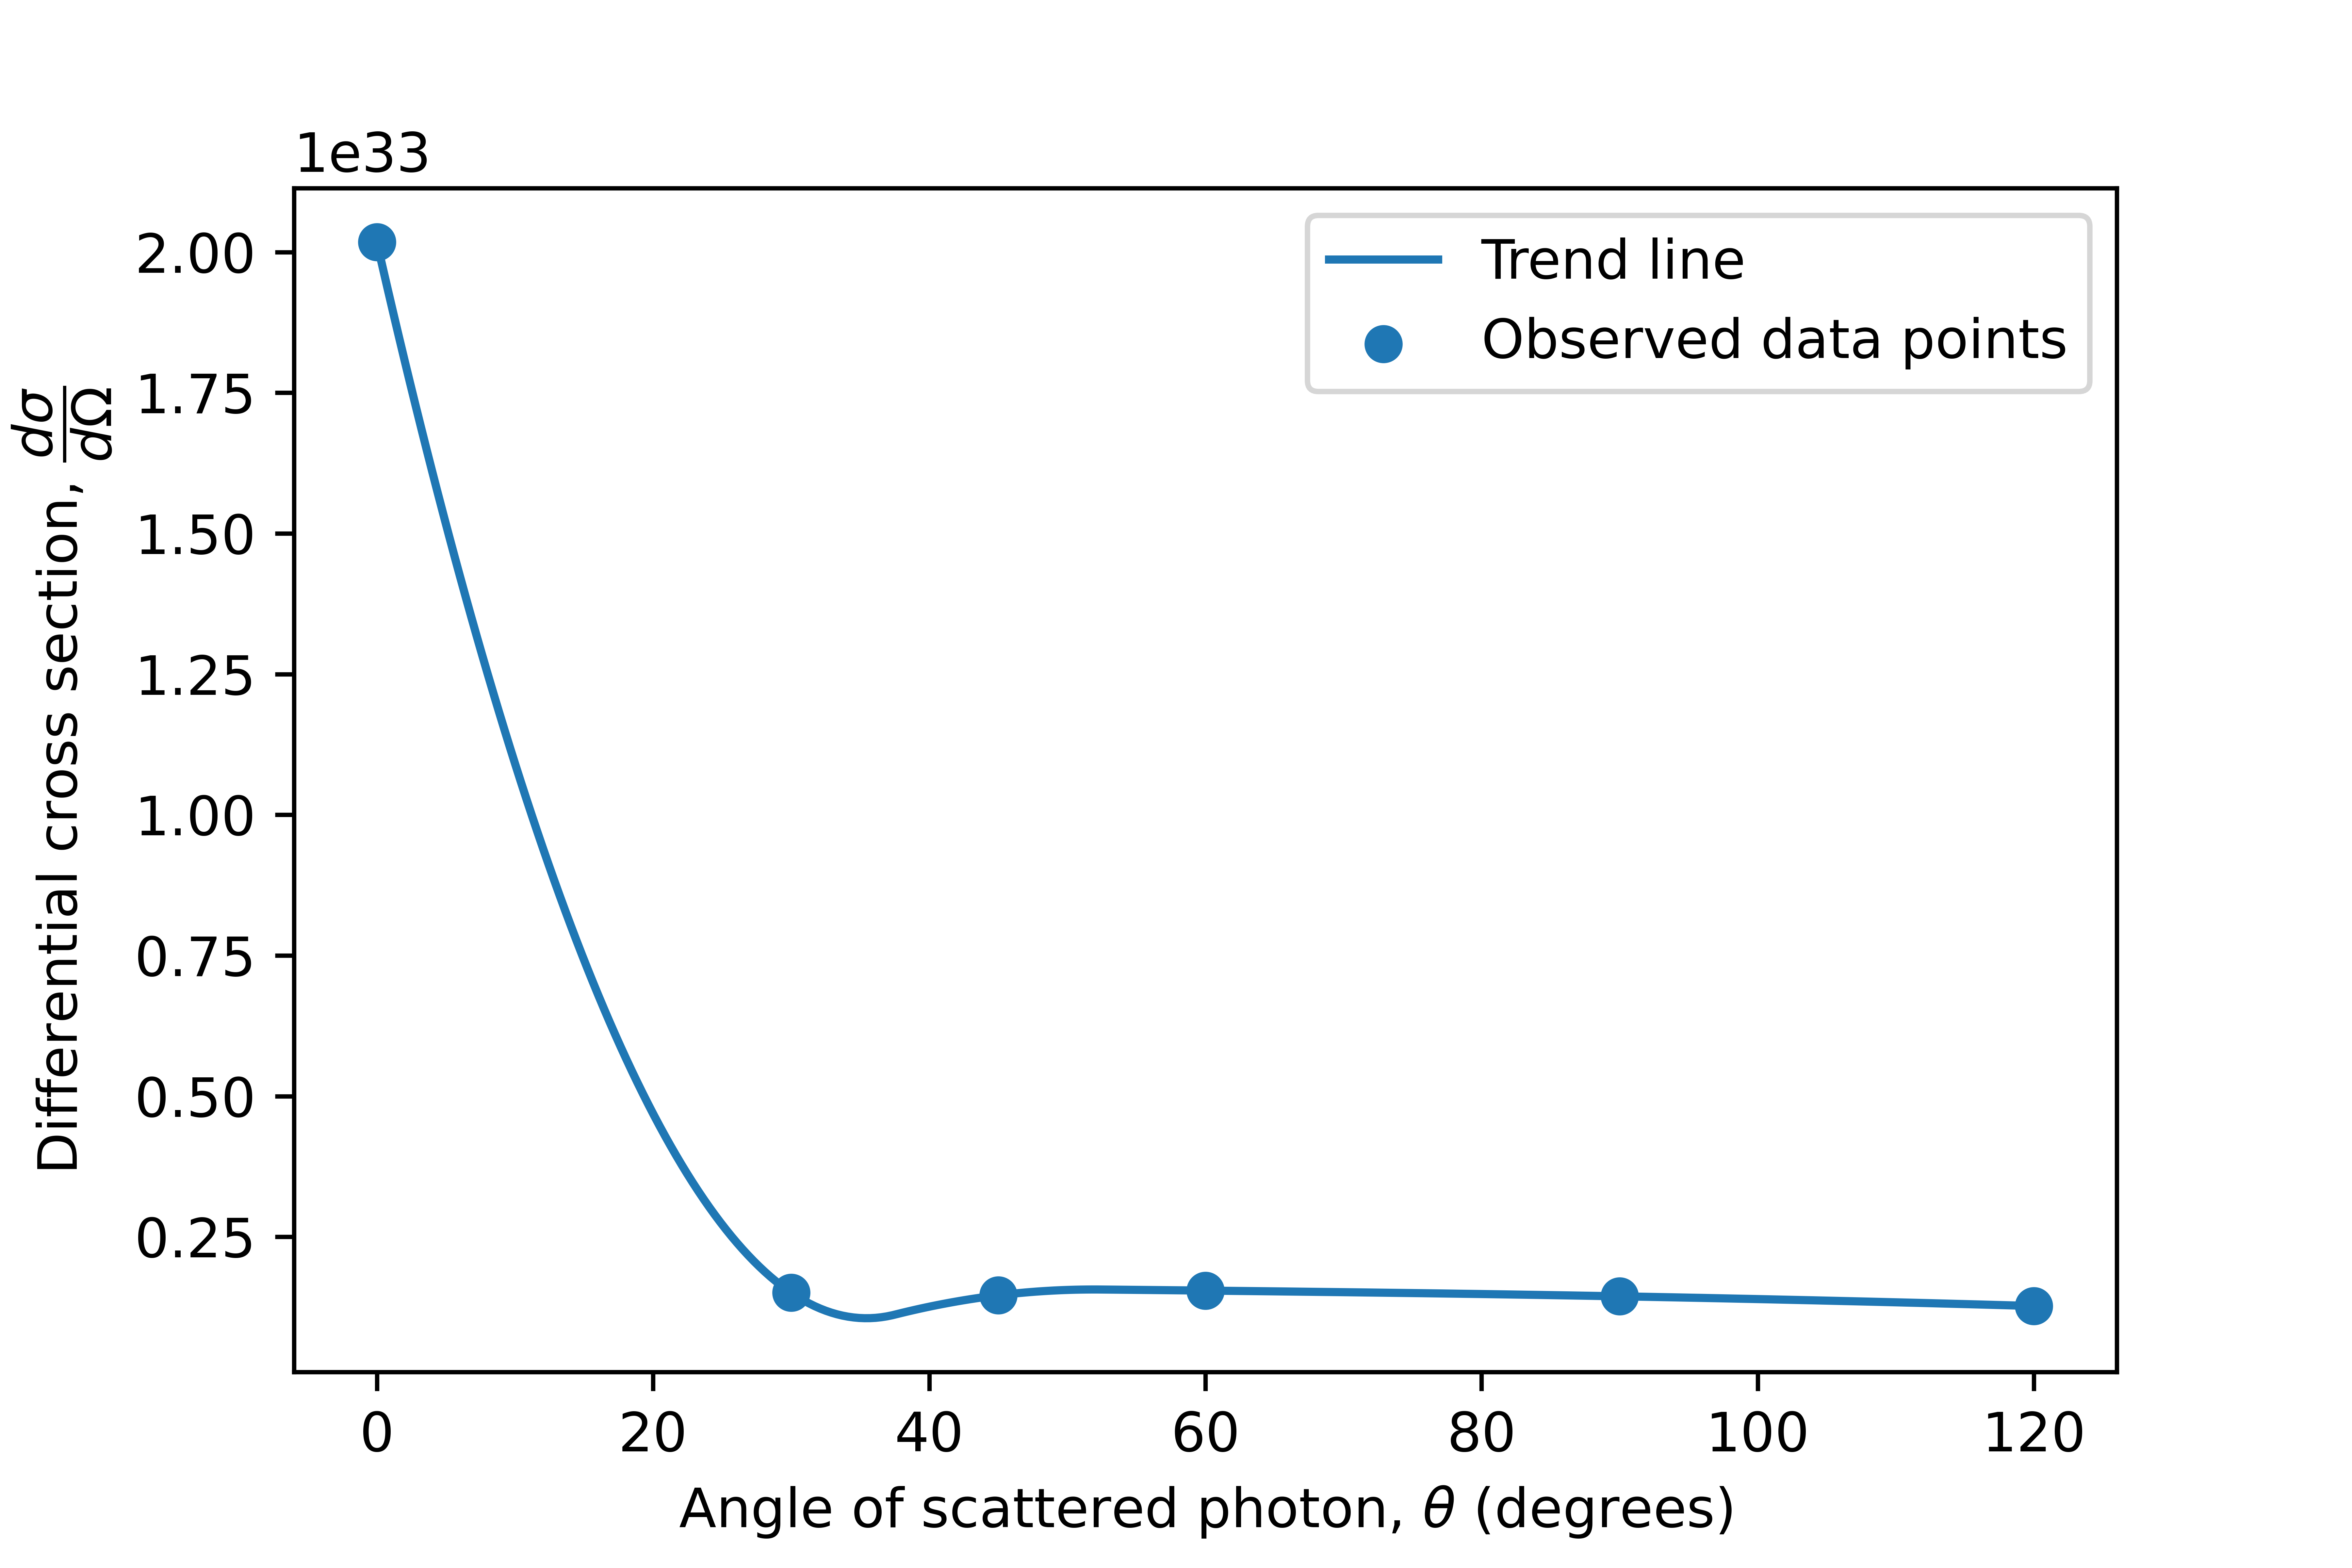
\includegraphics[scale = 0.56]{Figures/plot-al-C.png}
        \caption{Plot of differential cross-section with scattering angle for Aluminium}
        \label{fig:al-C}
    \end{figure}
    
    \subsection{Brass as the scattering body}
    The calibration curve is given in figure (\ref{fig:br-2}). The energy spectrum acquisition at various angles is given in figure (\ref{fig:br-1}). The corresponding plot of scattered energy $E_f$ against scattering angle $\theta$ is given in figure (\ref{fig:br-3}). The scattered energy, the differential cross-section, intensities and calibration factor are tabulated in table (\ref{tab:br}). The plot of differential cross-section with scattering angle is given in figure (\ref{fig:br-C}).
    \par
    From the table (\ref{tab:br}), the average calibration factor using equation (\ref{eq:calib}) is
    \begin{equation}
        \begin{split}
            C_{brass} &= \dfrac{1}{n} \sum_{\theta = 0}^{n} \dfrac{I_{\theta}}{\frac{d \sigma}{d \Omega}} \\
            &= \dfrac{1}{6} \times 1.611 \times 10^{33} \\
            &= \boxed{2.685 \times 10^{32}}
        \end{split}
    \end{equation}
    
    \begin{figure}
        \centering
        \hfill
        \begin{subfigure}[b]{0.48\textwidth}
            \centering
            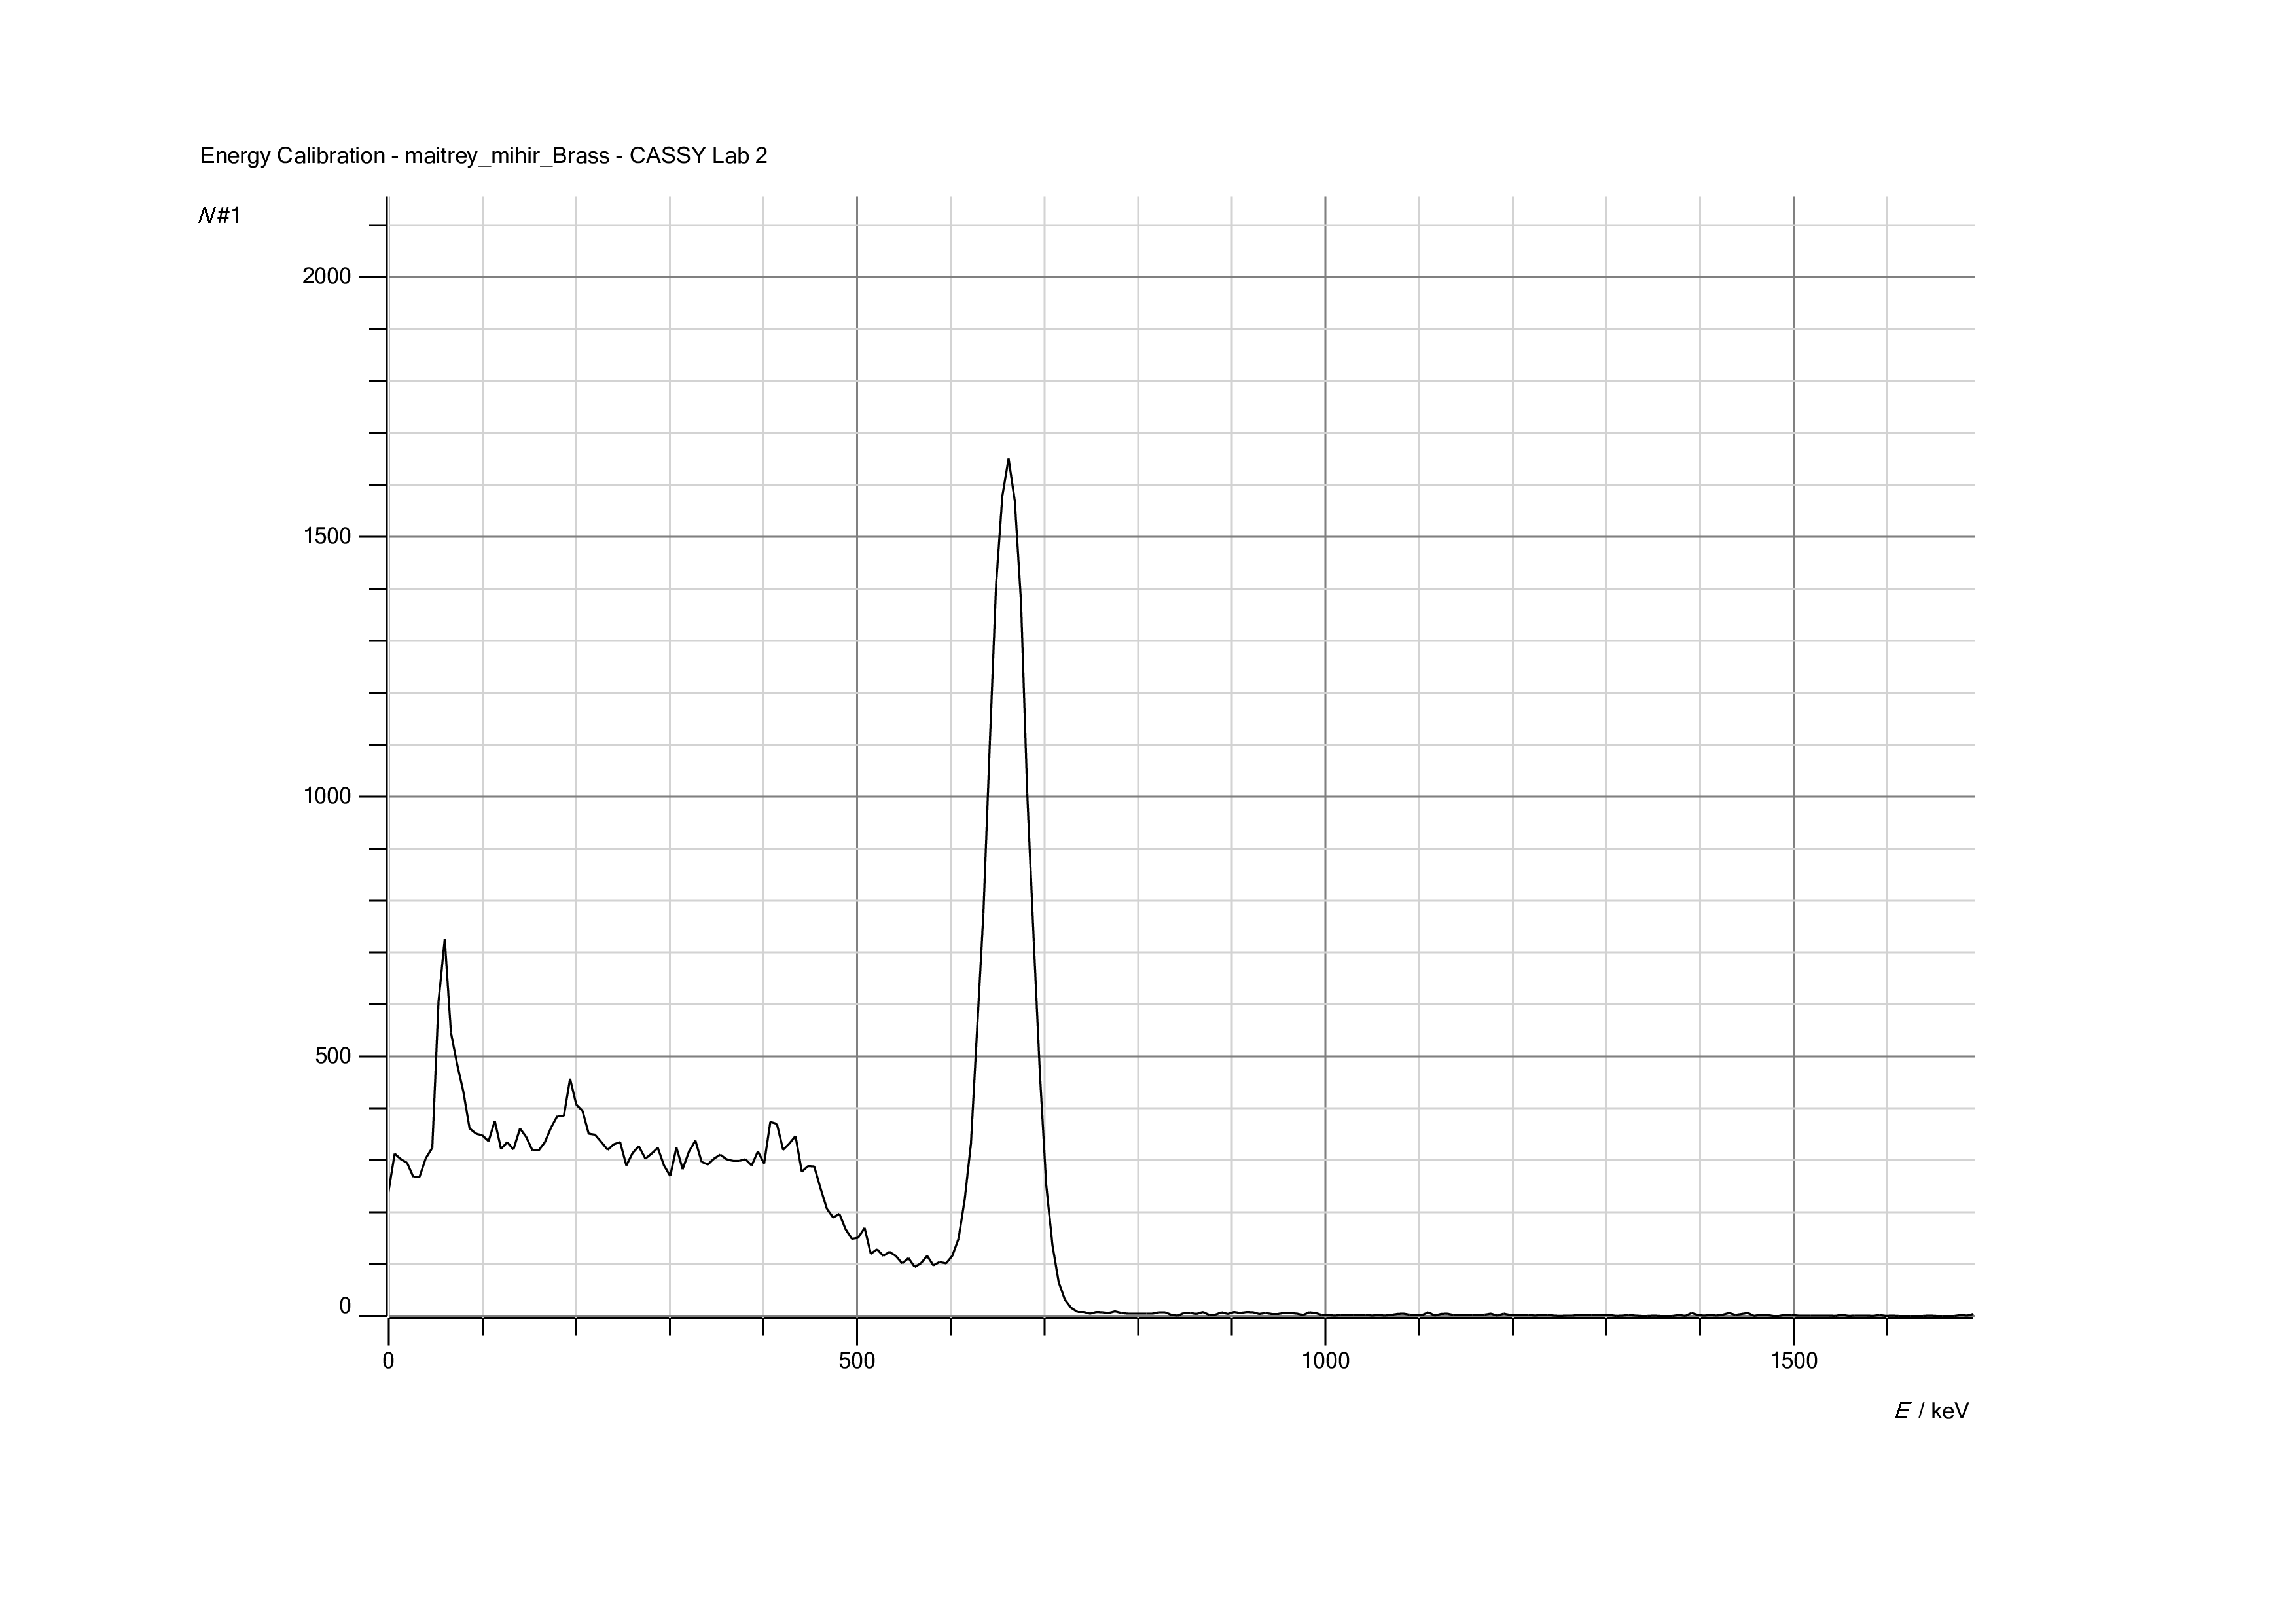
\includegraphics[scale = 0.069]{Figures/calib_Brass_diagram.png}
            \caption{Calibration plot}
            \label{fig:br-2}
        \end{subfigure}
        \begin{subfigure}[b]{0.48\textwidth}
            \centering
            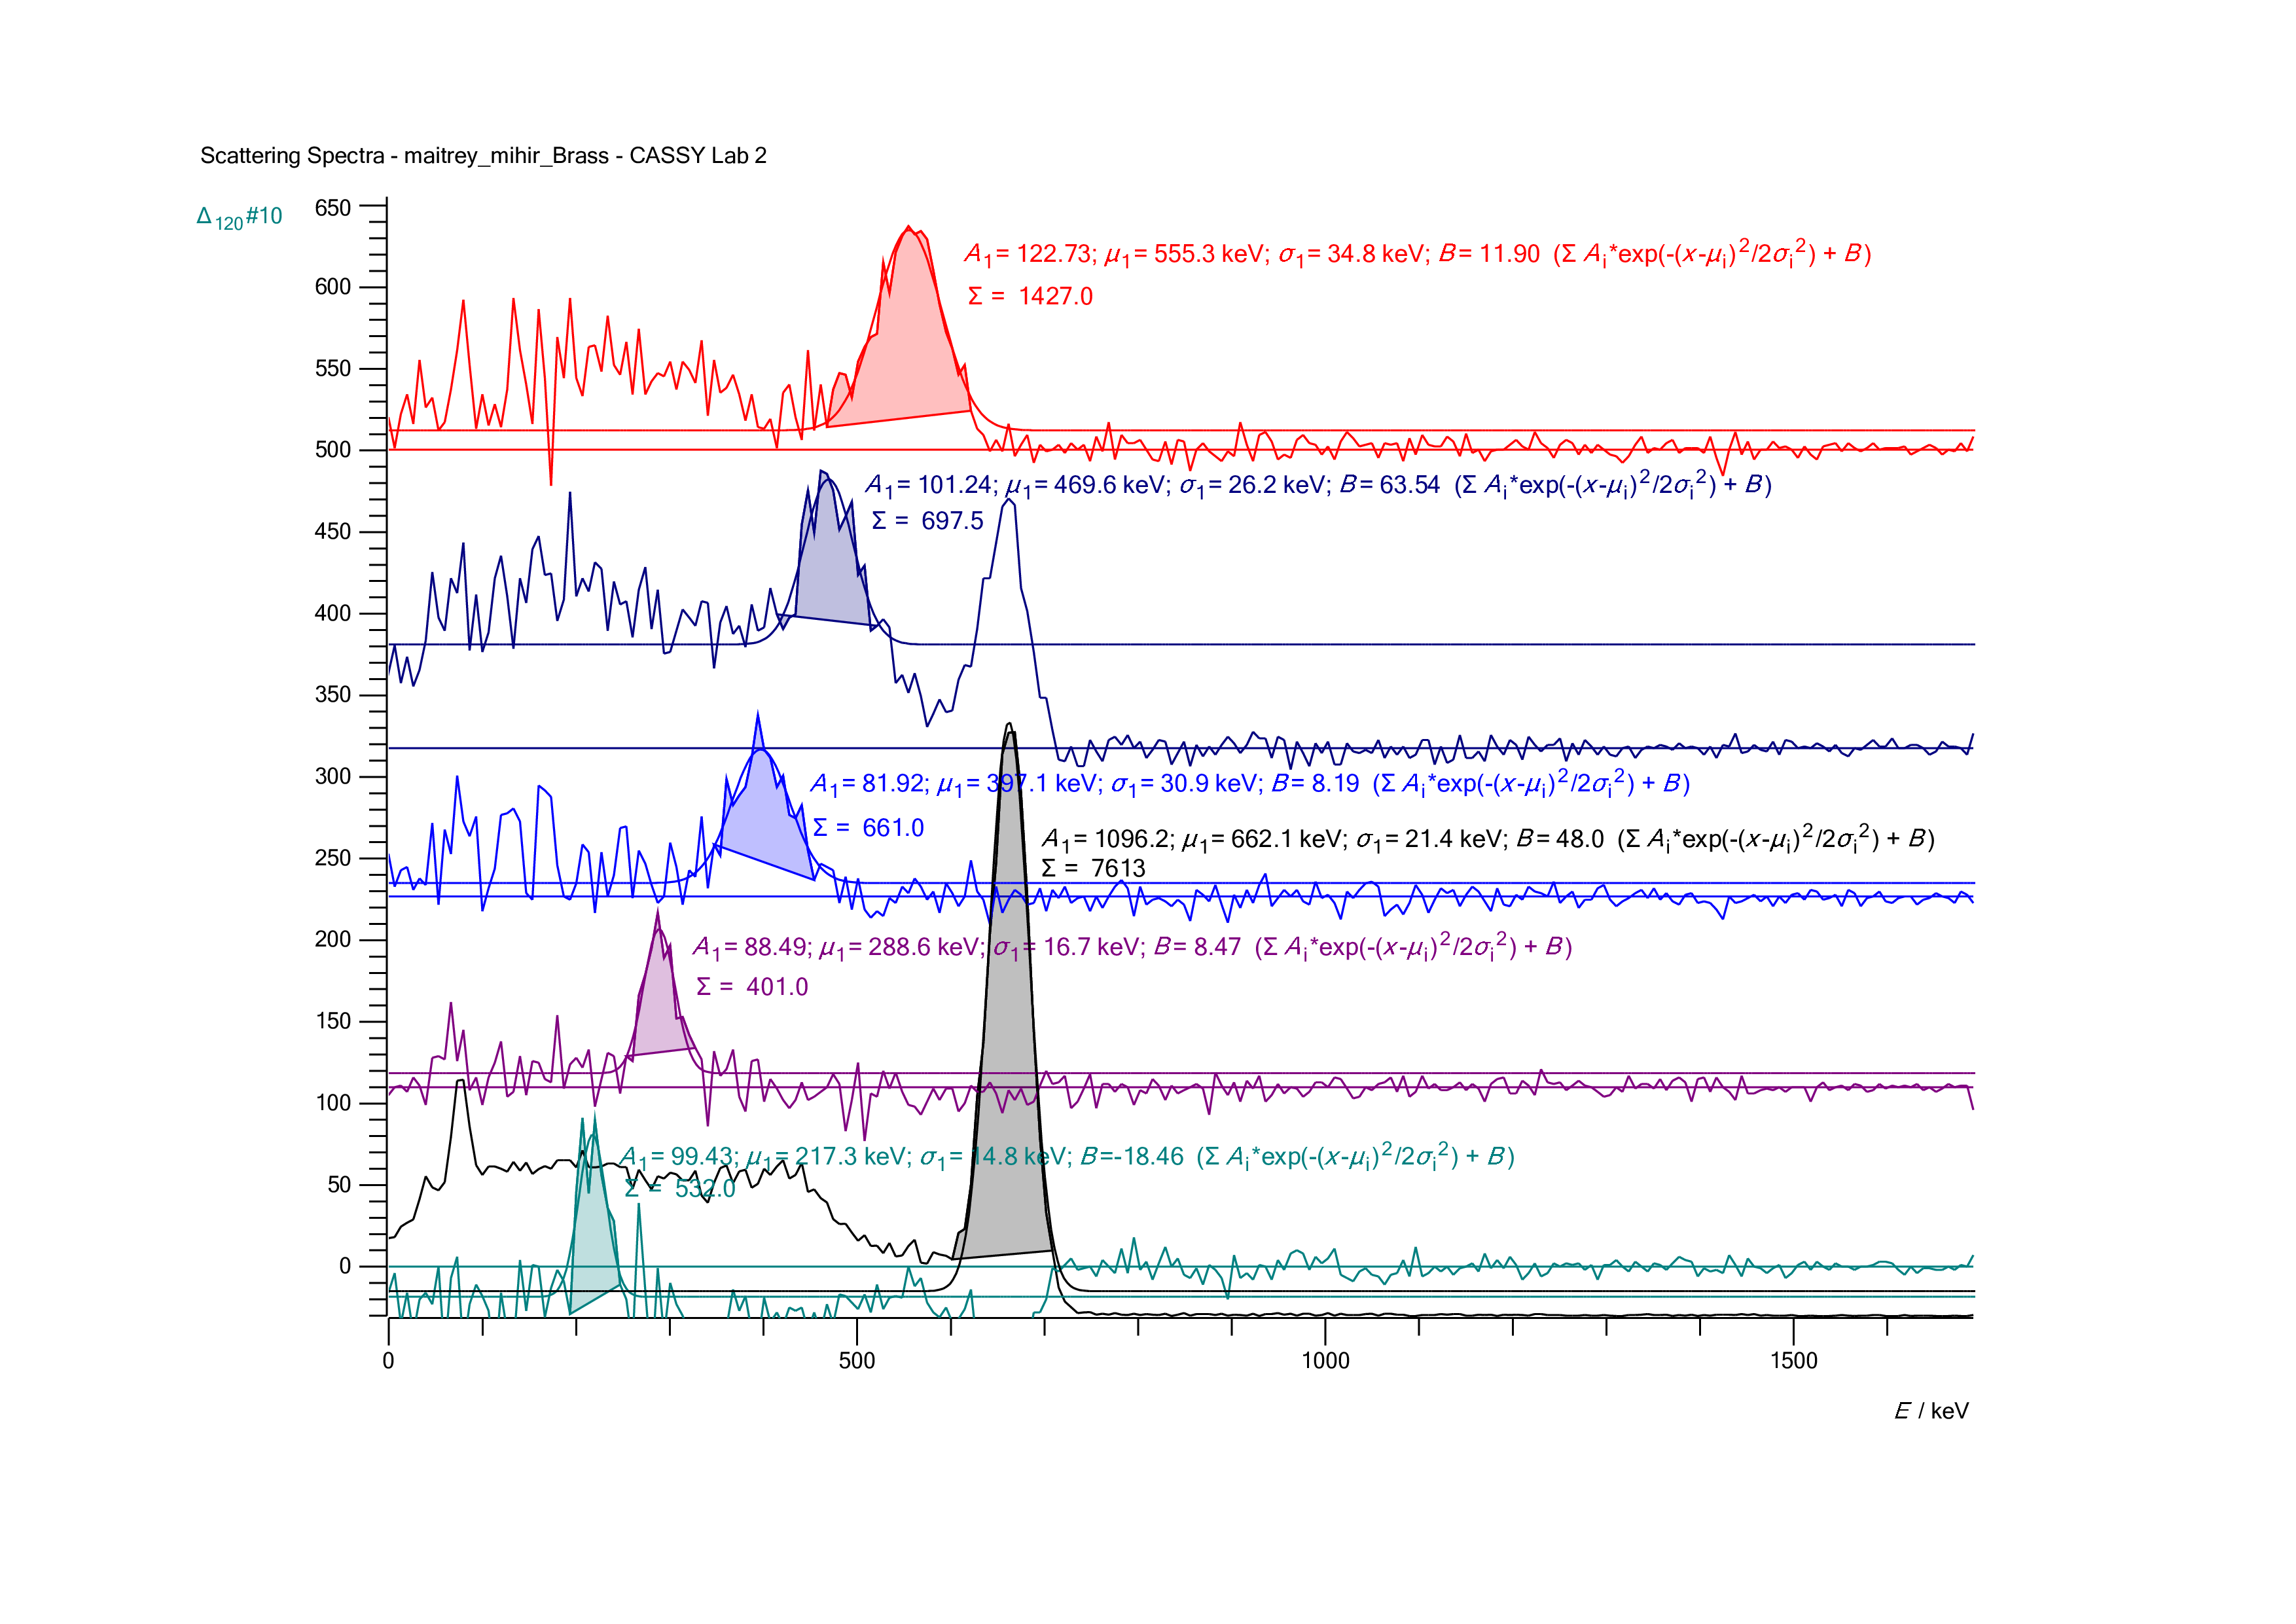
\includegraphics[scale = 0.069]{Figures/diagram_brass.png}
            \caption{Energy spectrum acquisition plot}
            \label{fig:br-1}
        \end{subfigure}
        \hfill
        \begin{subfigure}[b]{0.48\textwidth}
            \centering
            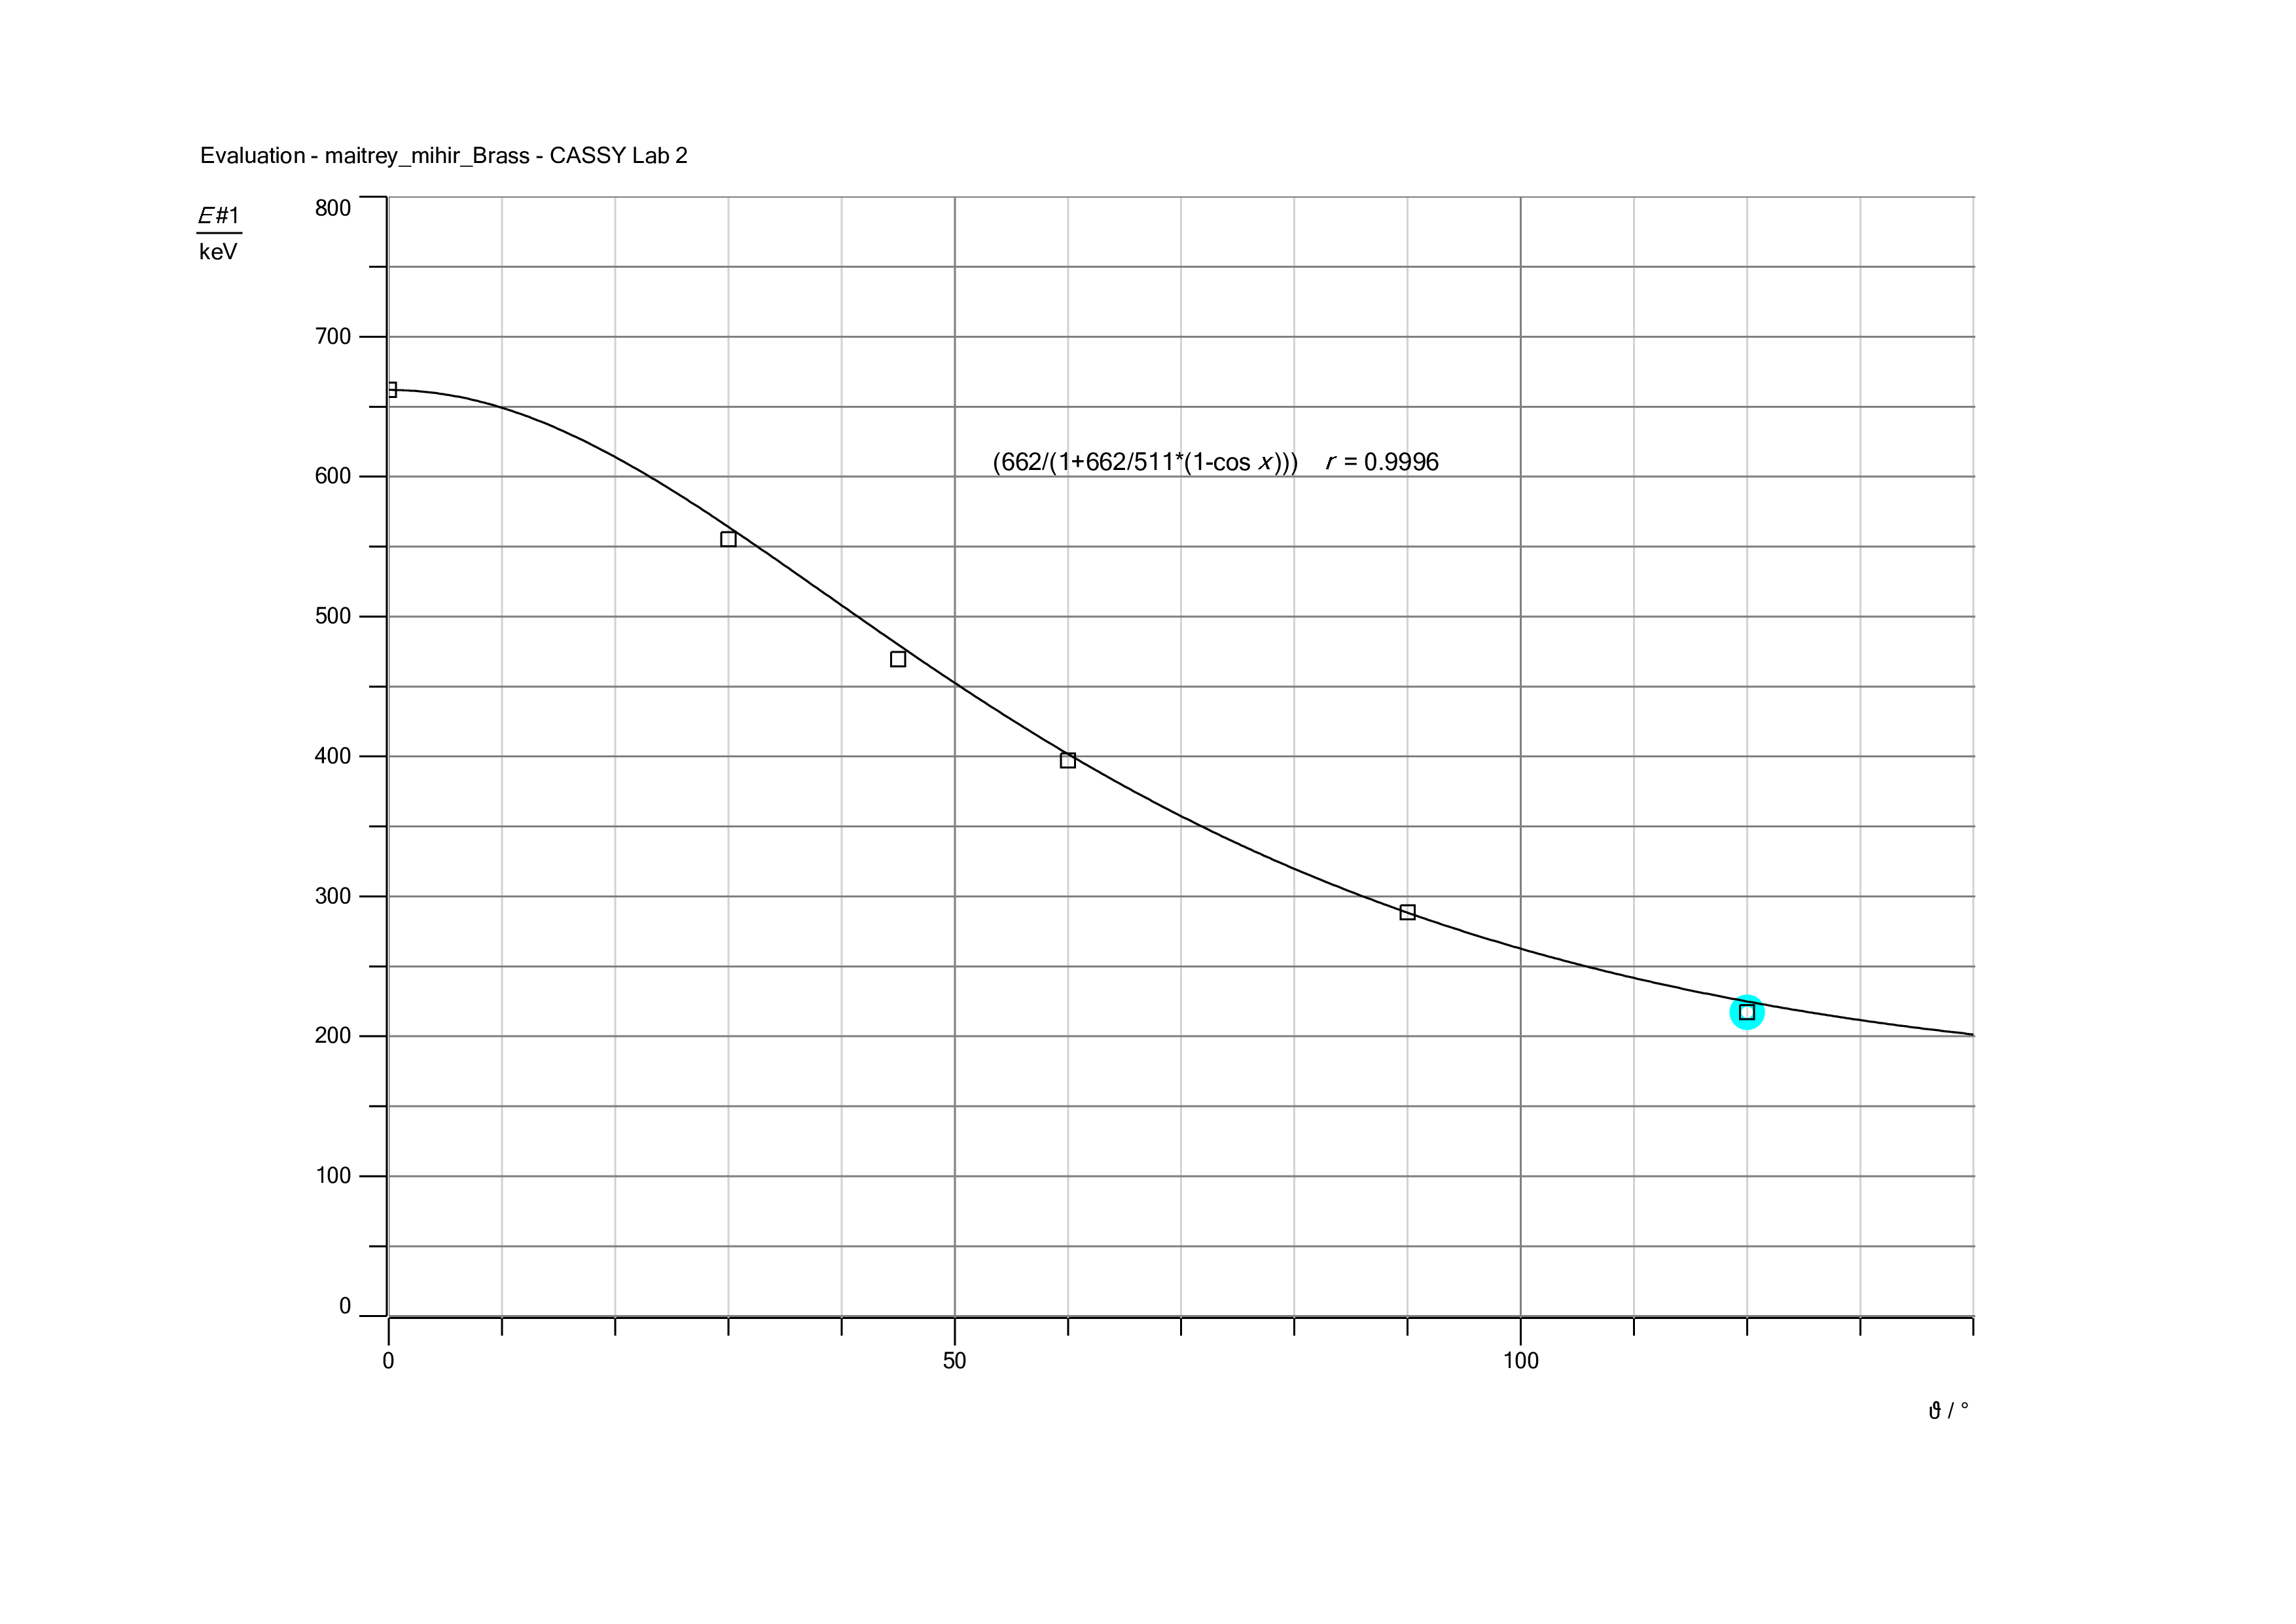
\includegraphics[scale = 0.069]{Figures/eval_brass_diagram.png}
            \caption{Plot of scattered energy with scattering angle}
            \label{fig:br-3}
        \end{subfigure}
            \caption{Calibration, energy spectrum acquisition and scattered energy versus scattering angle plots for Brass}
            \label{fig:br}
    \end{figure}
    

    \begin{table*}[]
    \caption{The scattered energy, the differential cross-section, intensities and the calibration factor for brass. The intensities are the area under the curve of the peak in the energy spectrum acquisition plots given in figure (\ref{fig:br-1})}
    \label{tab:br}
    \setlength{\tabcolsep}{15pt}
    \begin{tabular}{@{}ccccccc@{}}
    \toprule
    \begin{tabular}[c]{@{}c@{}}$\bm{\theta}$\\ (degrees)\end{tabular} &
    \begin{tabular}[c]{@{}c@{}}$\bm{E_f}$\\ ($\si{\kilo \electronvolt}$)\end{tabular} & 
    \begin{tabular}[c]{@{}c@{}}$\bm{E_f}$\\ ($\si{\joule}$)\end{tabular} &
    \begin{tabular}[c]{@{}c@{}}$\bm{\gamma}$\\ ($\si{\joule \second \squared \per \kilogram \per \metre}$) \end{tabular} & 
    \begin{tabular}[c]{@{}c@{}}\textbf{Differential}\\ \textbf{cross-section}\end{tabular} & $\bm{I_{\theta}}$ & 
    \begin{tabular}[c]{@{}c@{}}$\bm{C_{\theta}}$\\ ($\si{\steradian \per \metre \squared}$)\end{tabular} \\ \midrule
    0 & 662.1 & $1.059 \times 10^{-19}$ & $1.284 \times 10^{-06}$ & $7.998 \times 10^{-30}$ & 16138 & $9.519 \times 10^{32}$ \\
    30 & 555.3 &  $8.885 \times 10^{-20}$ & $1.082 \times 10^{-06}$ & $6.998 \times 10^{-30}$ & 1056 & $2.039 \times 10^{32}$ \\
    45 & 469.6 &  $7.514 \times 10^{-20}$ & $9.135 \times 10^{-07}$ & $5.998 \times 10^{-30}$ & 877 & $1.163 \times 10^{32}$ \\
    60 & 397.1 &  $6.354 \times 10^{-20}$ & $7.703 \times 10^{-07}$ & $4.998 \times 10^{-30}$ & 773 & $1.322 \times 10^{32}$ \\
    90 & 288.6 &  $4.618 \times 10^{-20}$ & $5.572 \times 10^{-07}$ & $3.999 \times 10^{-30}$ & 577.5 & $1.003 \times 10^{32}$ \\
    120 & 217.3 &  $3.477 \times 10^{-20}$ & $4.376 \times 10^{-07}$ & $4.998 \times 10^{-30}$ & 636 & $1.064 \times 10^{32}$ \\ \bottomrule
    \end{tabular}
    \end{table*}
    \begin{figure}
        \centering
        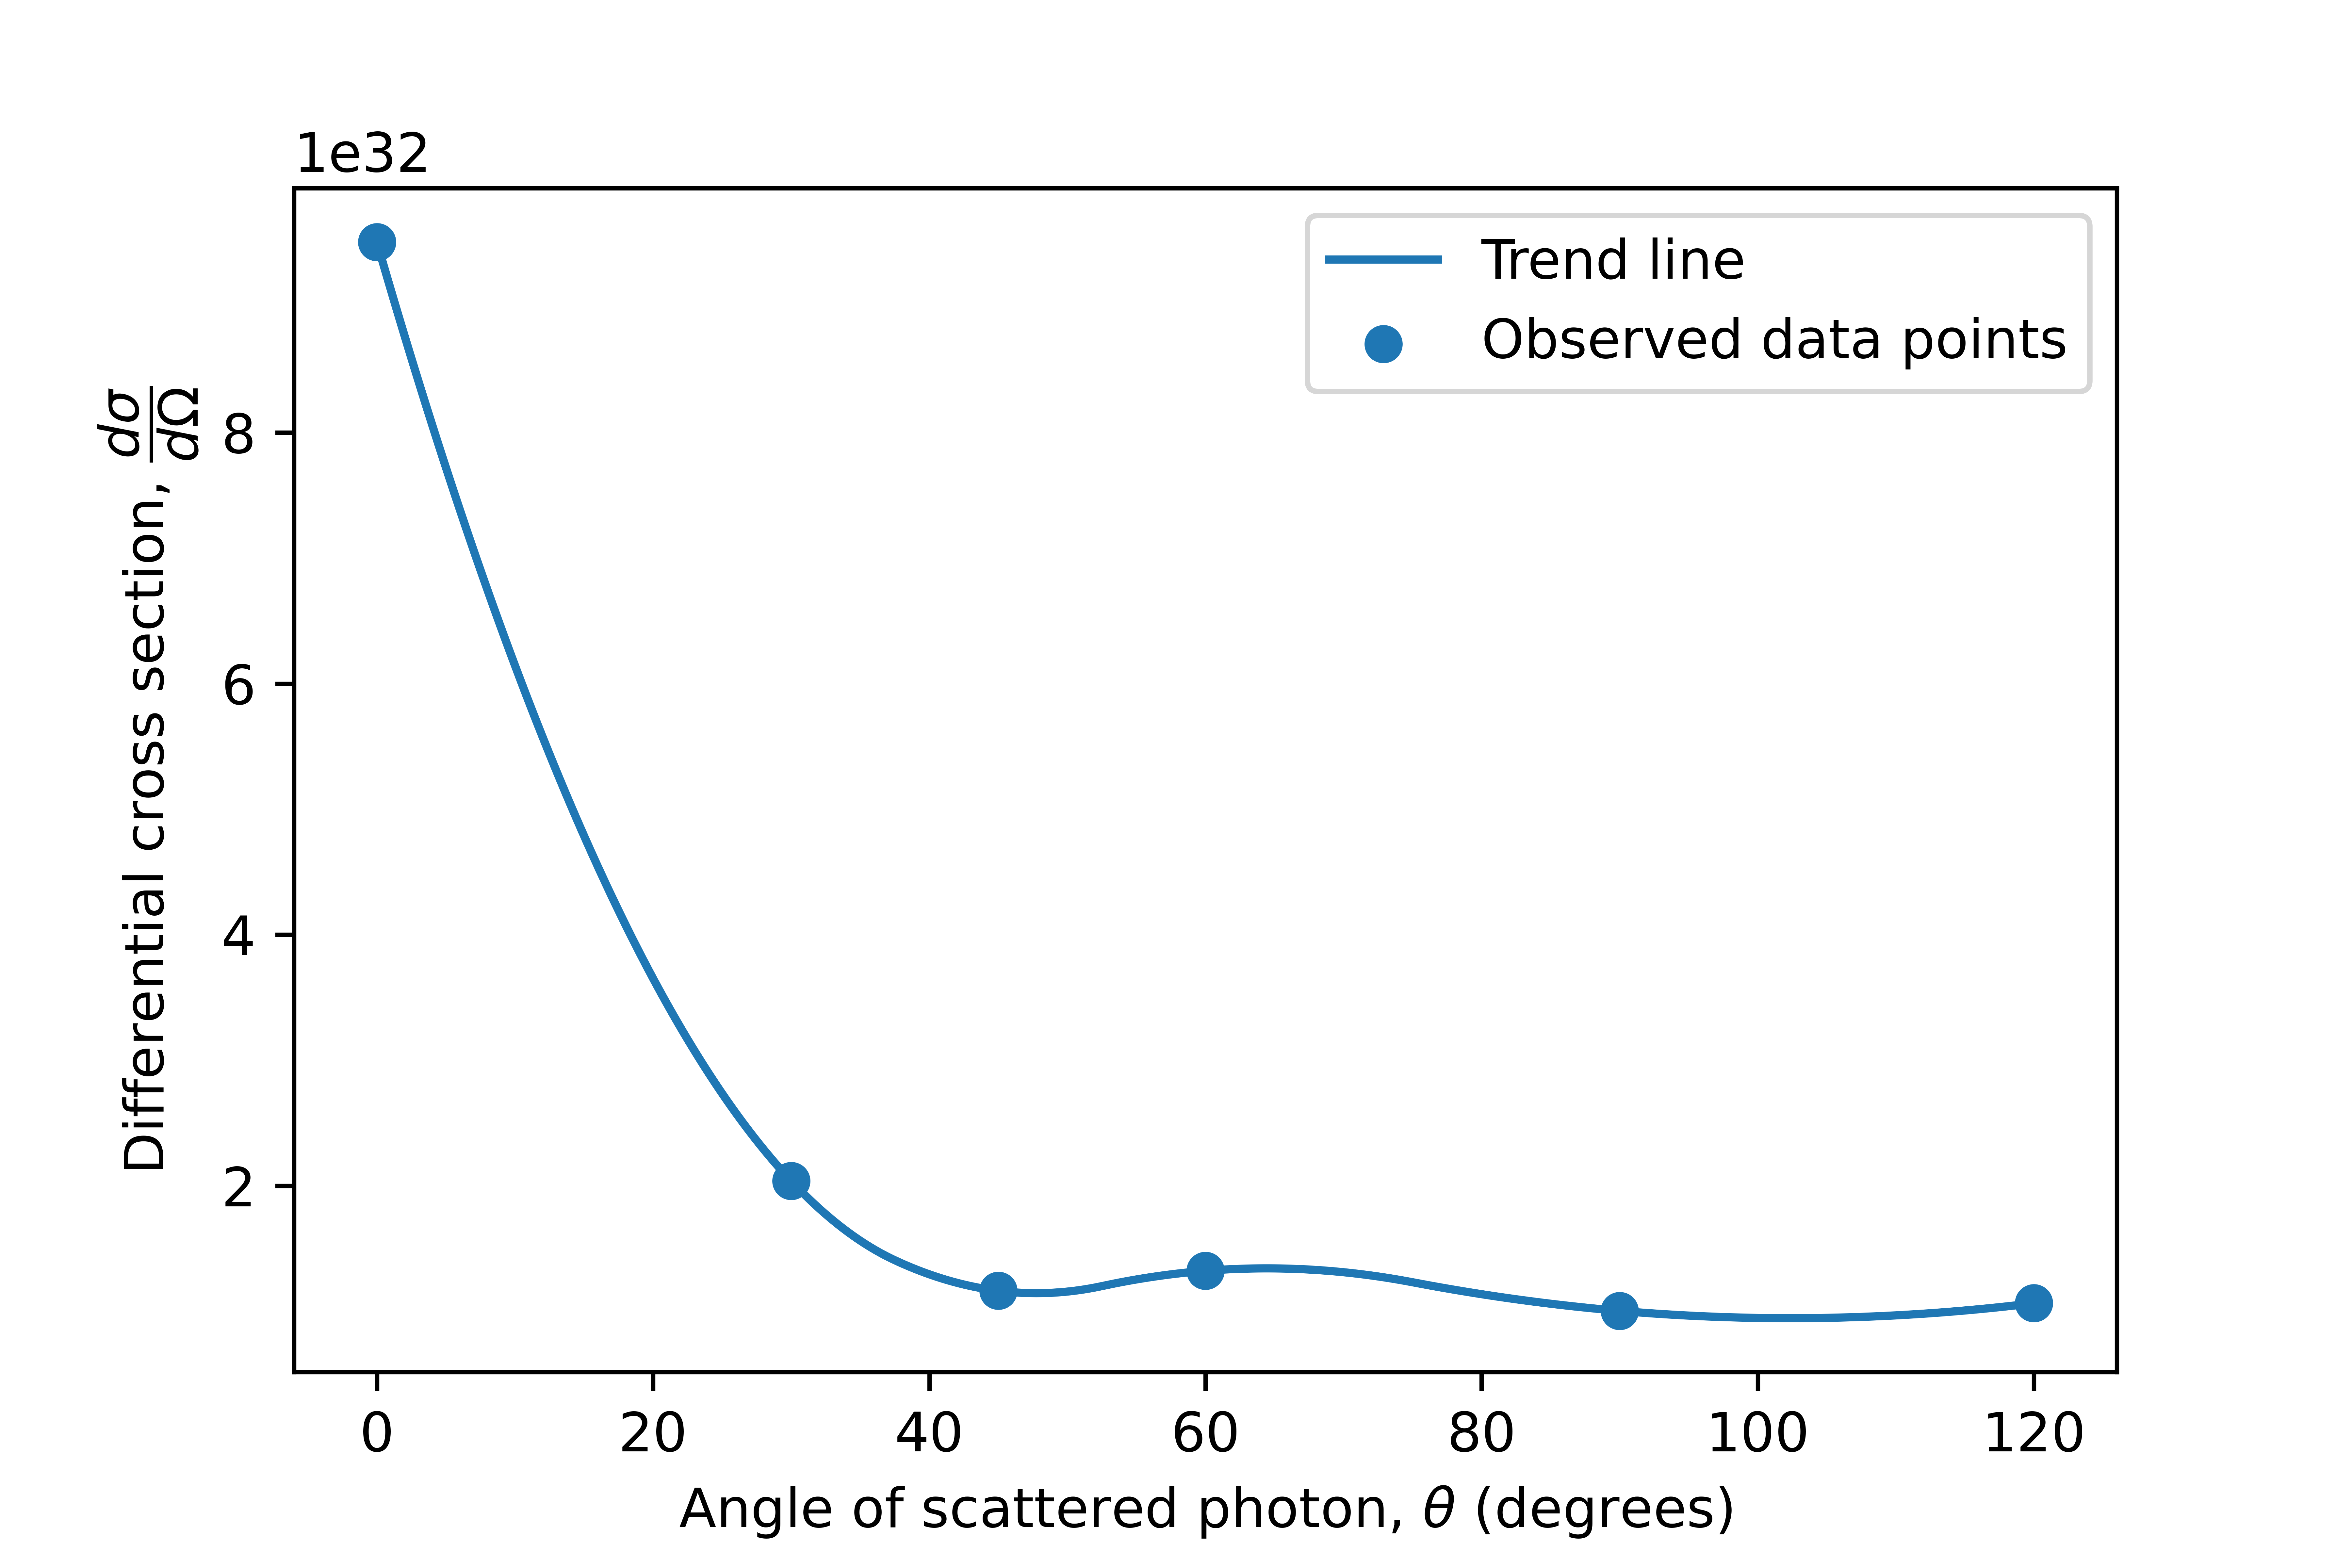
\includegraphics[scale = 0.56]{Figures/plot-brass-C.png}
        \caption{Plot of differential cross-section with scattering angle for brass}
        \label{fig:br-C}
    \end{figure}
    
\section{Error Analysis}
    \subsection{Aluminium as the scattering body}
    To calculate the error in the mean calibration factor, we recall theory of standard deviations. The standard deviation $\sigma_{Al}$ of a sample data is given by
    \begin{equation}
        \sigma_{Al} = \sqrt{\dfrac{\sum (x_i - \mu)^2}{N-1}}
    \end{equation}
    where $x_i$ is the $i$th observation, $\mu$ is the mean and $N$ is sample size. Putting in the corresponding values we get
    \begin{equation}
        \sigma_{Al} = 7.648 \times 10^{32}
    \end{equation}
    Now the standard error in mean is given by
    \begin{equation}
        \begin{split}
            \delta C_{Al} &= \dfrac{\sigma_{Al}}{\sqrt{N}} \\
            &= \dfrac{7.648 \times 10^{32}}{\sqrt{6}} \\
            &= \boxed{3.122 \times 10^{32}}
        \end{split}
    \end{equation}
    \subsection{Brass as the scattering body}
    The standard deviation $\sigma_{brass}$ of a sample data is given by
    \begin{equation}
        \sigma_{brass} = \sqrt{\dfrac{\sum (x_i - \mu)^2}{N-1}}
    \end{equation}
    where $x_i$ is the $i$th observation, $\mu$ is the mean and $N$ is sample size. Putting in the corresponding values we get
    \begin{equation}
        \sigma_{brass} = 3.369 \times 10^{32}
    \end{equation}
    Now the standard error in mean is given by
    \begin{equation}
        \begin{split}
            \delta C_{brass} &= \dfrac{\sigma_{brass}}{\sqrt{N}} \\
            &= \dfrac{3.369 \times 10^{32}}{\sqrt{6}} \\
            &= \boxed{1.375 \times 10^{32}}
        \end{split}
    \end{equation}

\section{Results}
    \begin{enumerate}
        \item The calibration factor for Aluminium was obtained as $C_{Al} = \SI[separate-uncertainty=true]{4.569 \pm 3.122e32}{\steradian \per \metre \squared}$.
        \item The calibration factor for brass was obtained as $C_{brass} = \SI[separate-uncertainty=true]{2.685 \pm 1.375e32}{\steradian \per \metre \squared}$.
    \end{enumerate}
    
\section{Discussions}
    \begin{enumerate}
        \item Energy of the scattered photon decreases with increase in angle, hence the wavelength increases. This implies that change in wavelength decreases with increasing angle.
        \item Calibration factor for brass was lower than Al because of the presence of more free electrons in Al. This could also be seen in the plots as Al has more counts than brass for all angles.
        \item The plot for scattering energy versus scattering angle could be fit to the theoretical equation, and hence was validated.
        \item Different peaks like Compton edge, photopeak were also identified in the spectrograph obtained in each case.
        \item Magnetic Compton scattering is an extension of the previously mentioned technique which involves the magnetisation of a crystal sample hit with high energy, circularly polarised photons. By measuring the scattered photons' energy and reversing the magnetisation of the sample, two different Compton profiles are generated (one for spin up momenta and one for spin down momenta). Taking the difference between these two profiles gives the magnetic Compton profile (MCP).
        \item Since magnetic Compton scattering is incoherent (there is no phase relationship between the scattered photons), the MCP is representative of the bulk properties of the sample and is a probe of the ground state. This means that the MCP is ideal for comparison with theoretical techniques such as density functional theory. The area under the MCP is directly proportional to the spin moment of the system and so, when combined with total moment measurements methods (such as SQUID magnetometry), can be used to isolate both the spin and orbital contributions to the total moment of a system. The shape of the MCP also yields insight into the origin of the magnetism in the system.
        \item Inverse Compton scattering is important in astrophysics. In X-ray astronomy, the accretion disk surrounding a black hole is presumed to produce a thermal spectrum. The lower energy photons produced from this spectrum are scattered to higher energies by relativistic electrons in the surrounding corona.
        \item Non-linear inverse Compton scattering (NICS) is the scattering of multiple low-energy photons, given by an intense electromagnetic field, in a high-energy photon (X-ray or gamma ray) during the interaction with a charged particle, such as an electron. It is also called non-linear Compton scattering and multiphoton Compton scattering. It is the non-linear version of inverse Compton scattering in which the conditions for multiphoton absorption by the charged particle are reached due to a very intense electromagnetic field, for example the one produced by a laser.
    \end{enumerate}

\section{Precautions}
    \begin{enumerate}
        \item The lead block should be placed such that no direct photons reach the detector, while also not blocking any scattered photons.
        \item Care must be take while performing the Gaussian fit.
        \item Manually setting the calibration can give wrong results as peaks could lie in between channels.
        \item The setup should be left undisturbed during the experiment.
        \item Nearby unknown sources could also alter the results of experiments.
    \end{enumerate}
\section{Conclusions}
    \begin{enumerate}
        \item We were able to calibrate the detector using a mixed source.
        \item We successfully studied Compton effect using a Cs-137 source and observed the difference for two scattering bodies, namely Aluminium and Brass.
    \end{enumerate}





\end{document}
%
% ****** End of file apssamp.tex ******
